\section{Supplementary Materials}
\label{SuppMaterials}
\setlength{\parindent}{20pt}
\justifying

\noindent
\def\arraystretch{0.8}

% BLP
\begin{figure}[!htbp]
    \begin{center}
        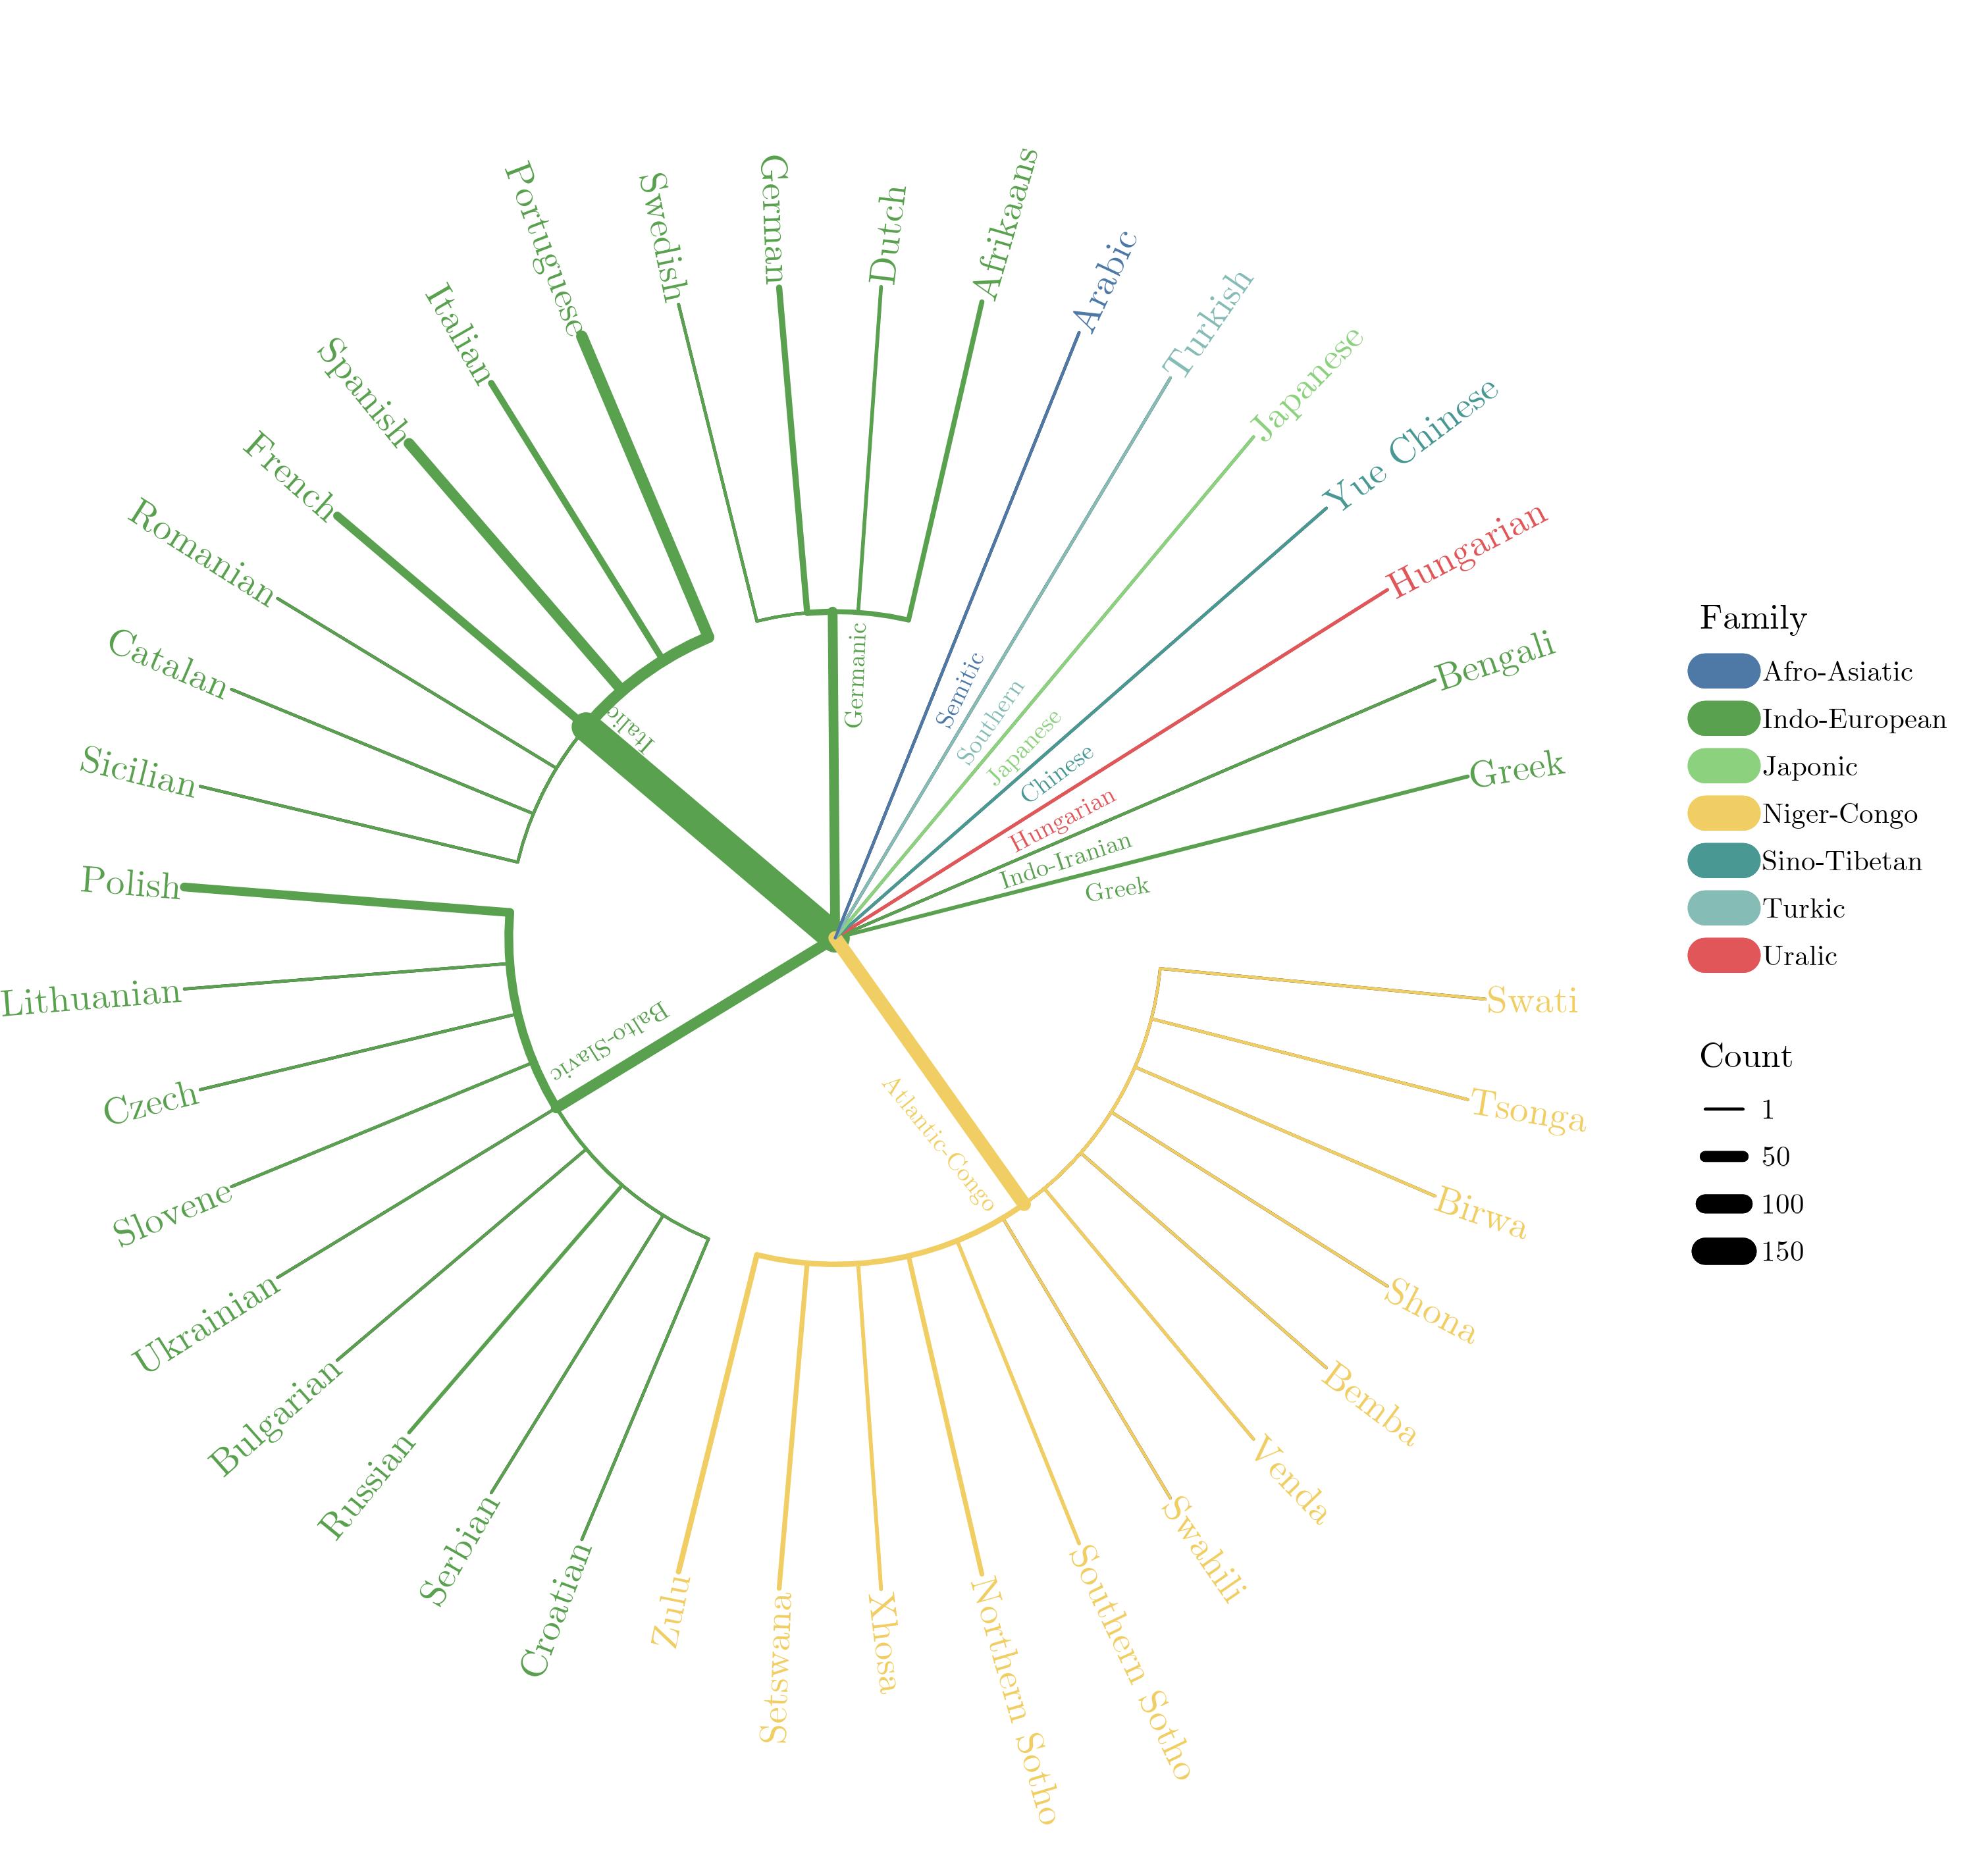
\includegraphics[width=0.52\textwidth]{Figures/exp1_languages.png}
    \end{center}
    \caption[]{\justifying Tree plot showcasing the range of language backgrounds of participants in experiment 1. The colours indicate the different language families. The inner ring holds the various branches of those families, each of those ending in individual language on the outer ring. Line thickness indicates the density of each element.}
    \label{exp1_BLPtree}
\end{figure}

\begin{figure}[!htbp]
    \begin{center}
        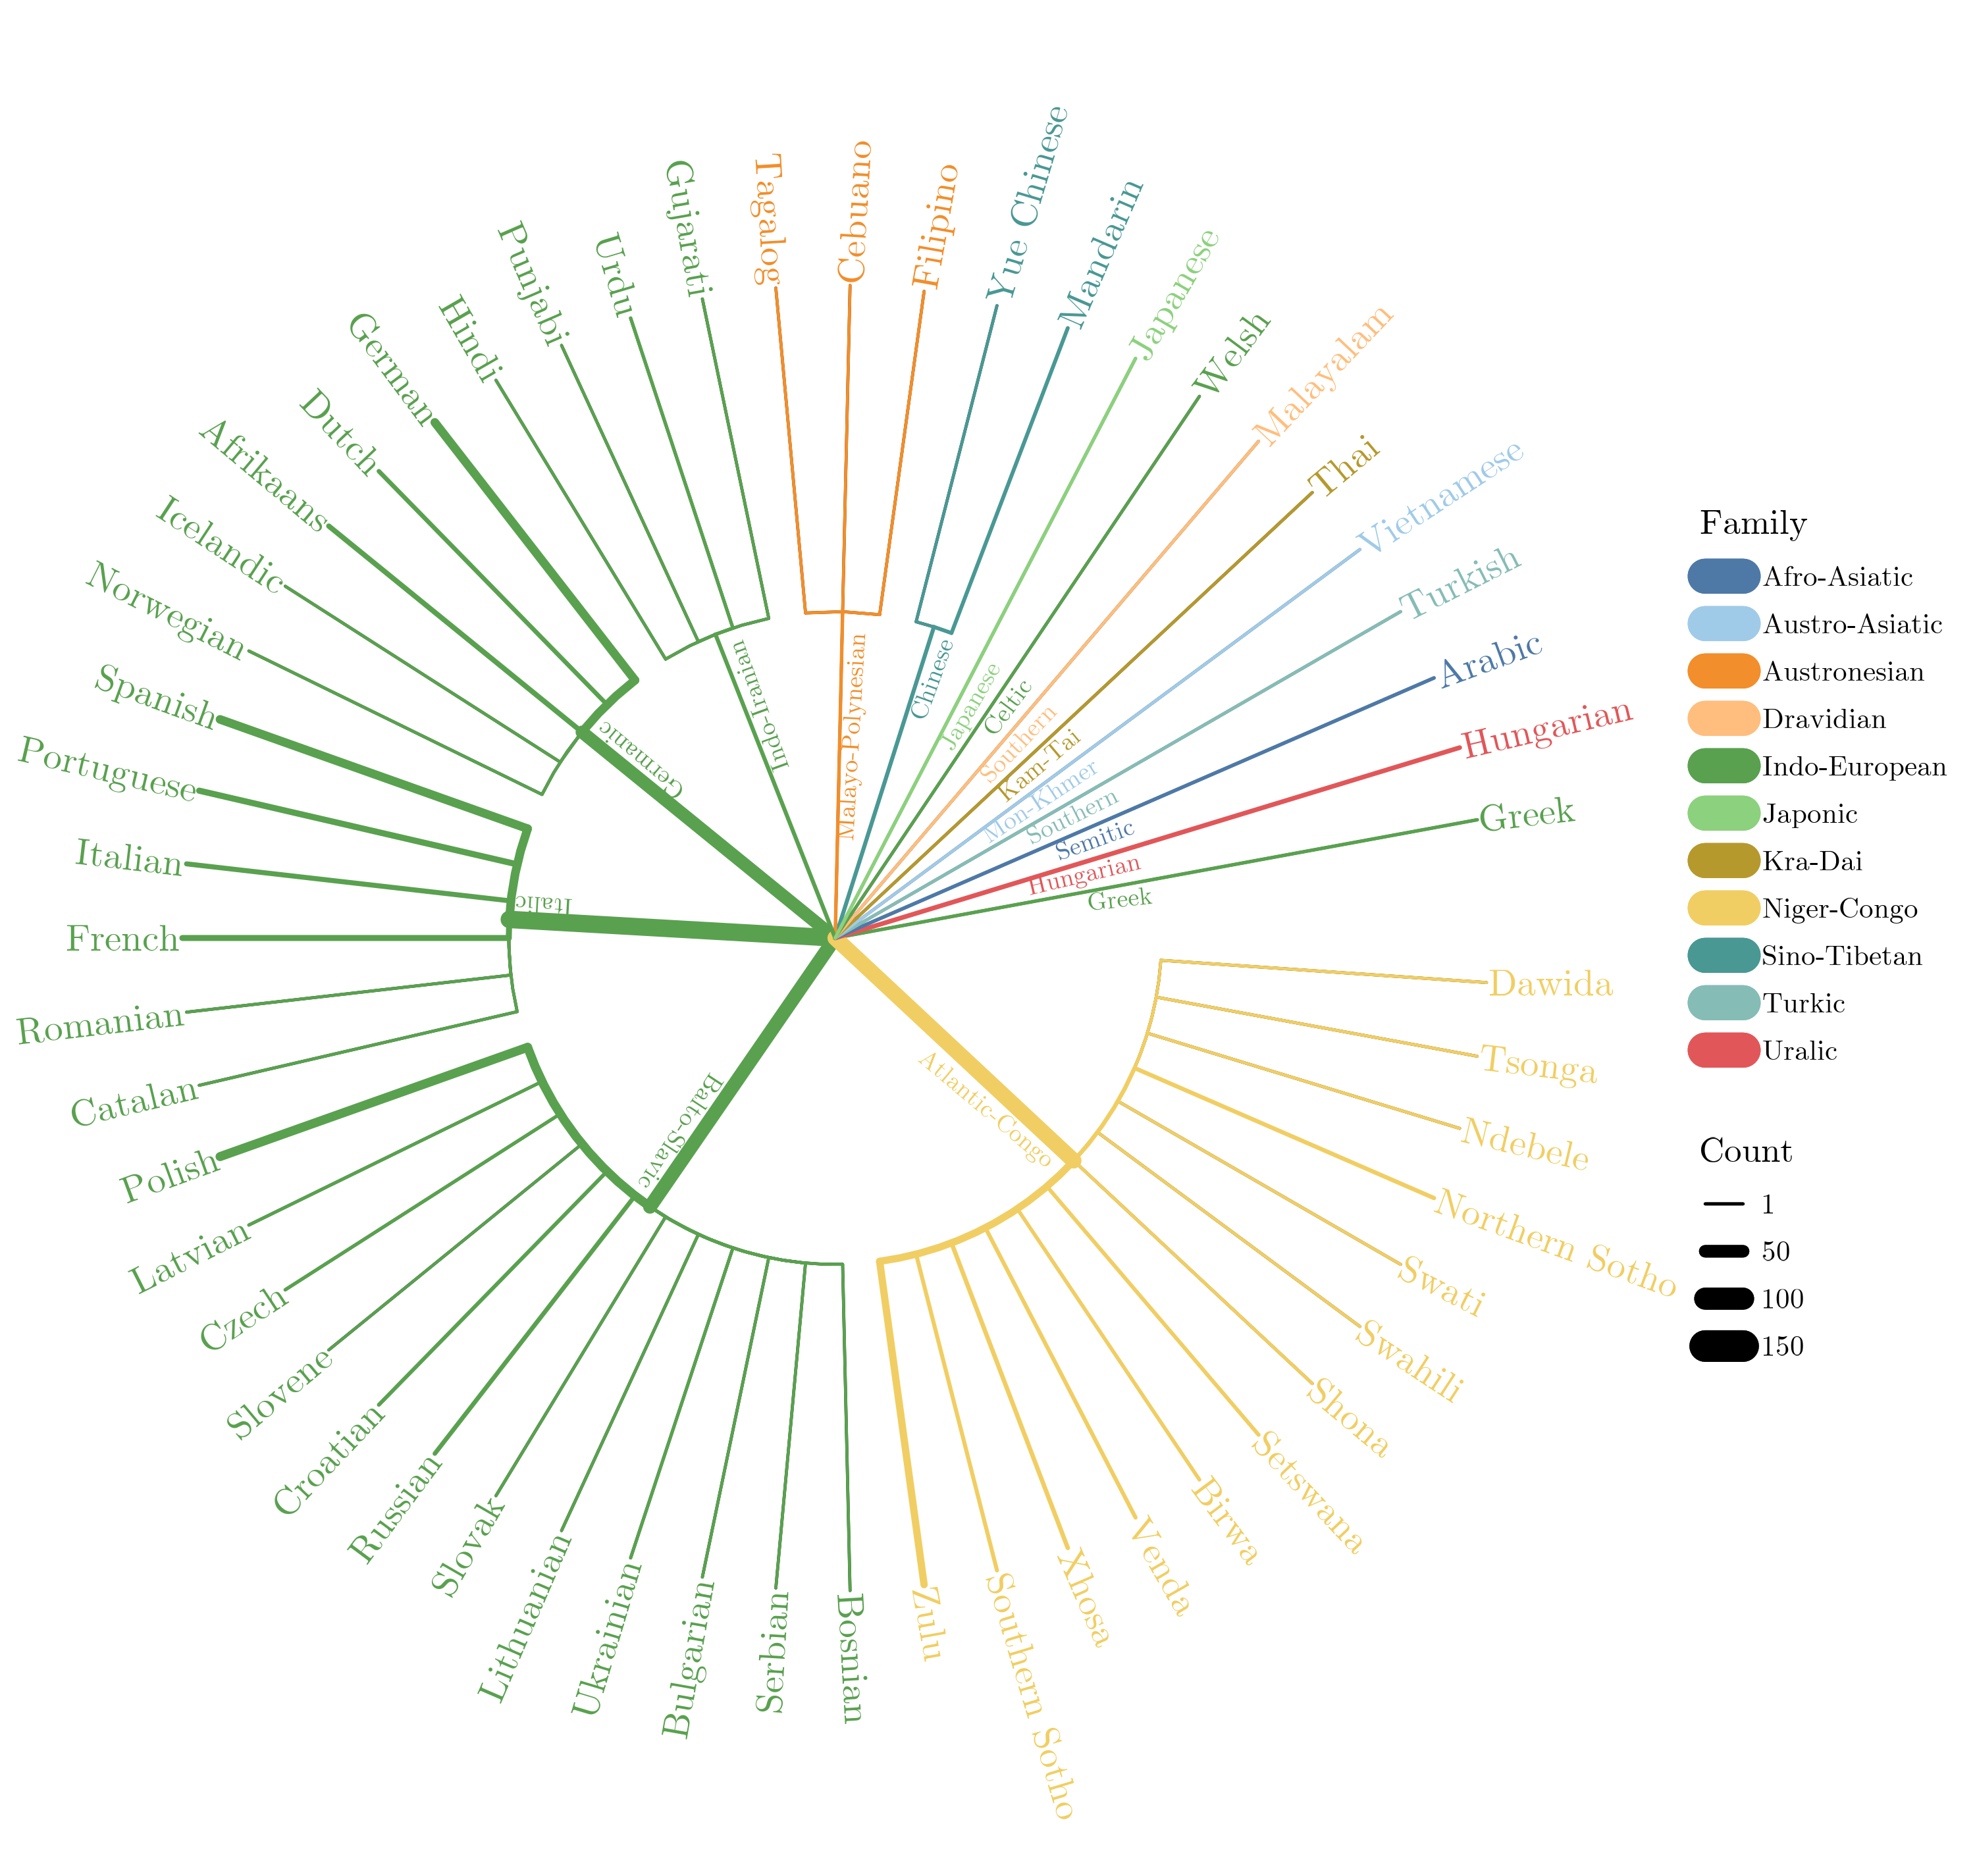
\includegraphics[width=0.52\textwidth]{Figures/exp2_languages.png}
    \end{center}
    \caption[]{\justifying Tree plot showcasing the range of language backgrounds of participants in experiment 2. The colours indicate the different language families. The inner ring holds the various branches of those families, each of those ending in individual language on the outer ring. Line thickness indicates the density of each element.}
    \label{exp2_BLPtree}
\end{figure}

\begin{figure}[!htbp]
    \begin{center}
        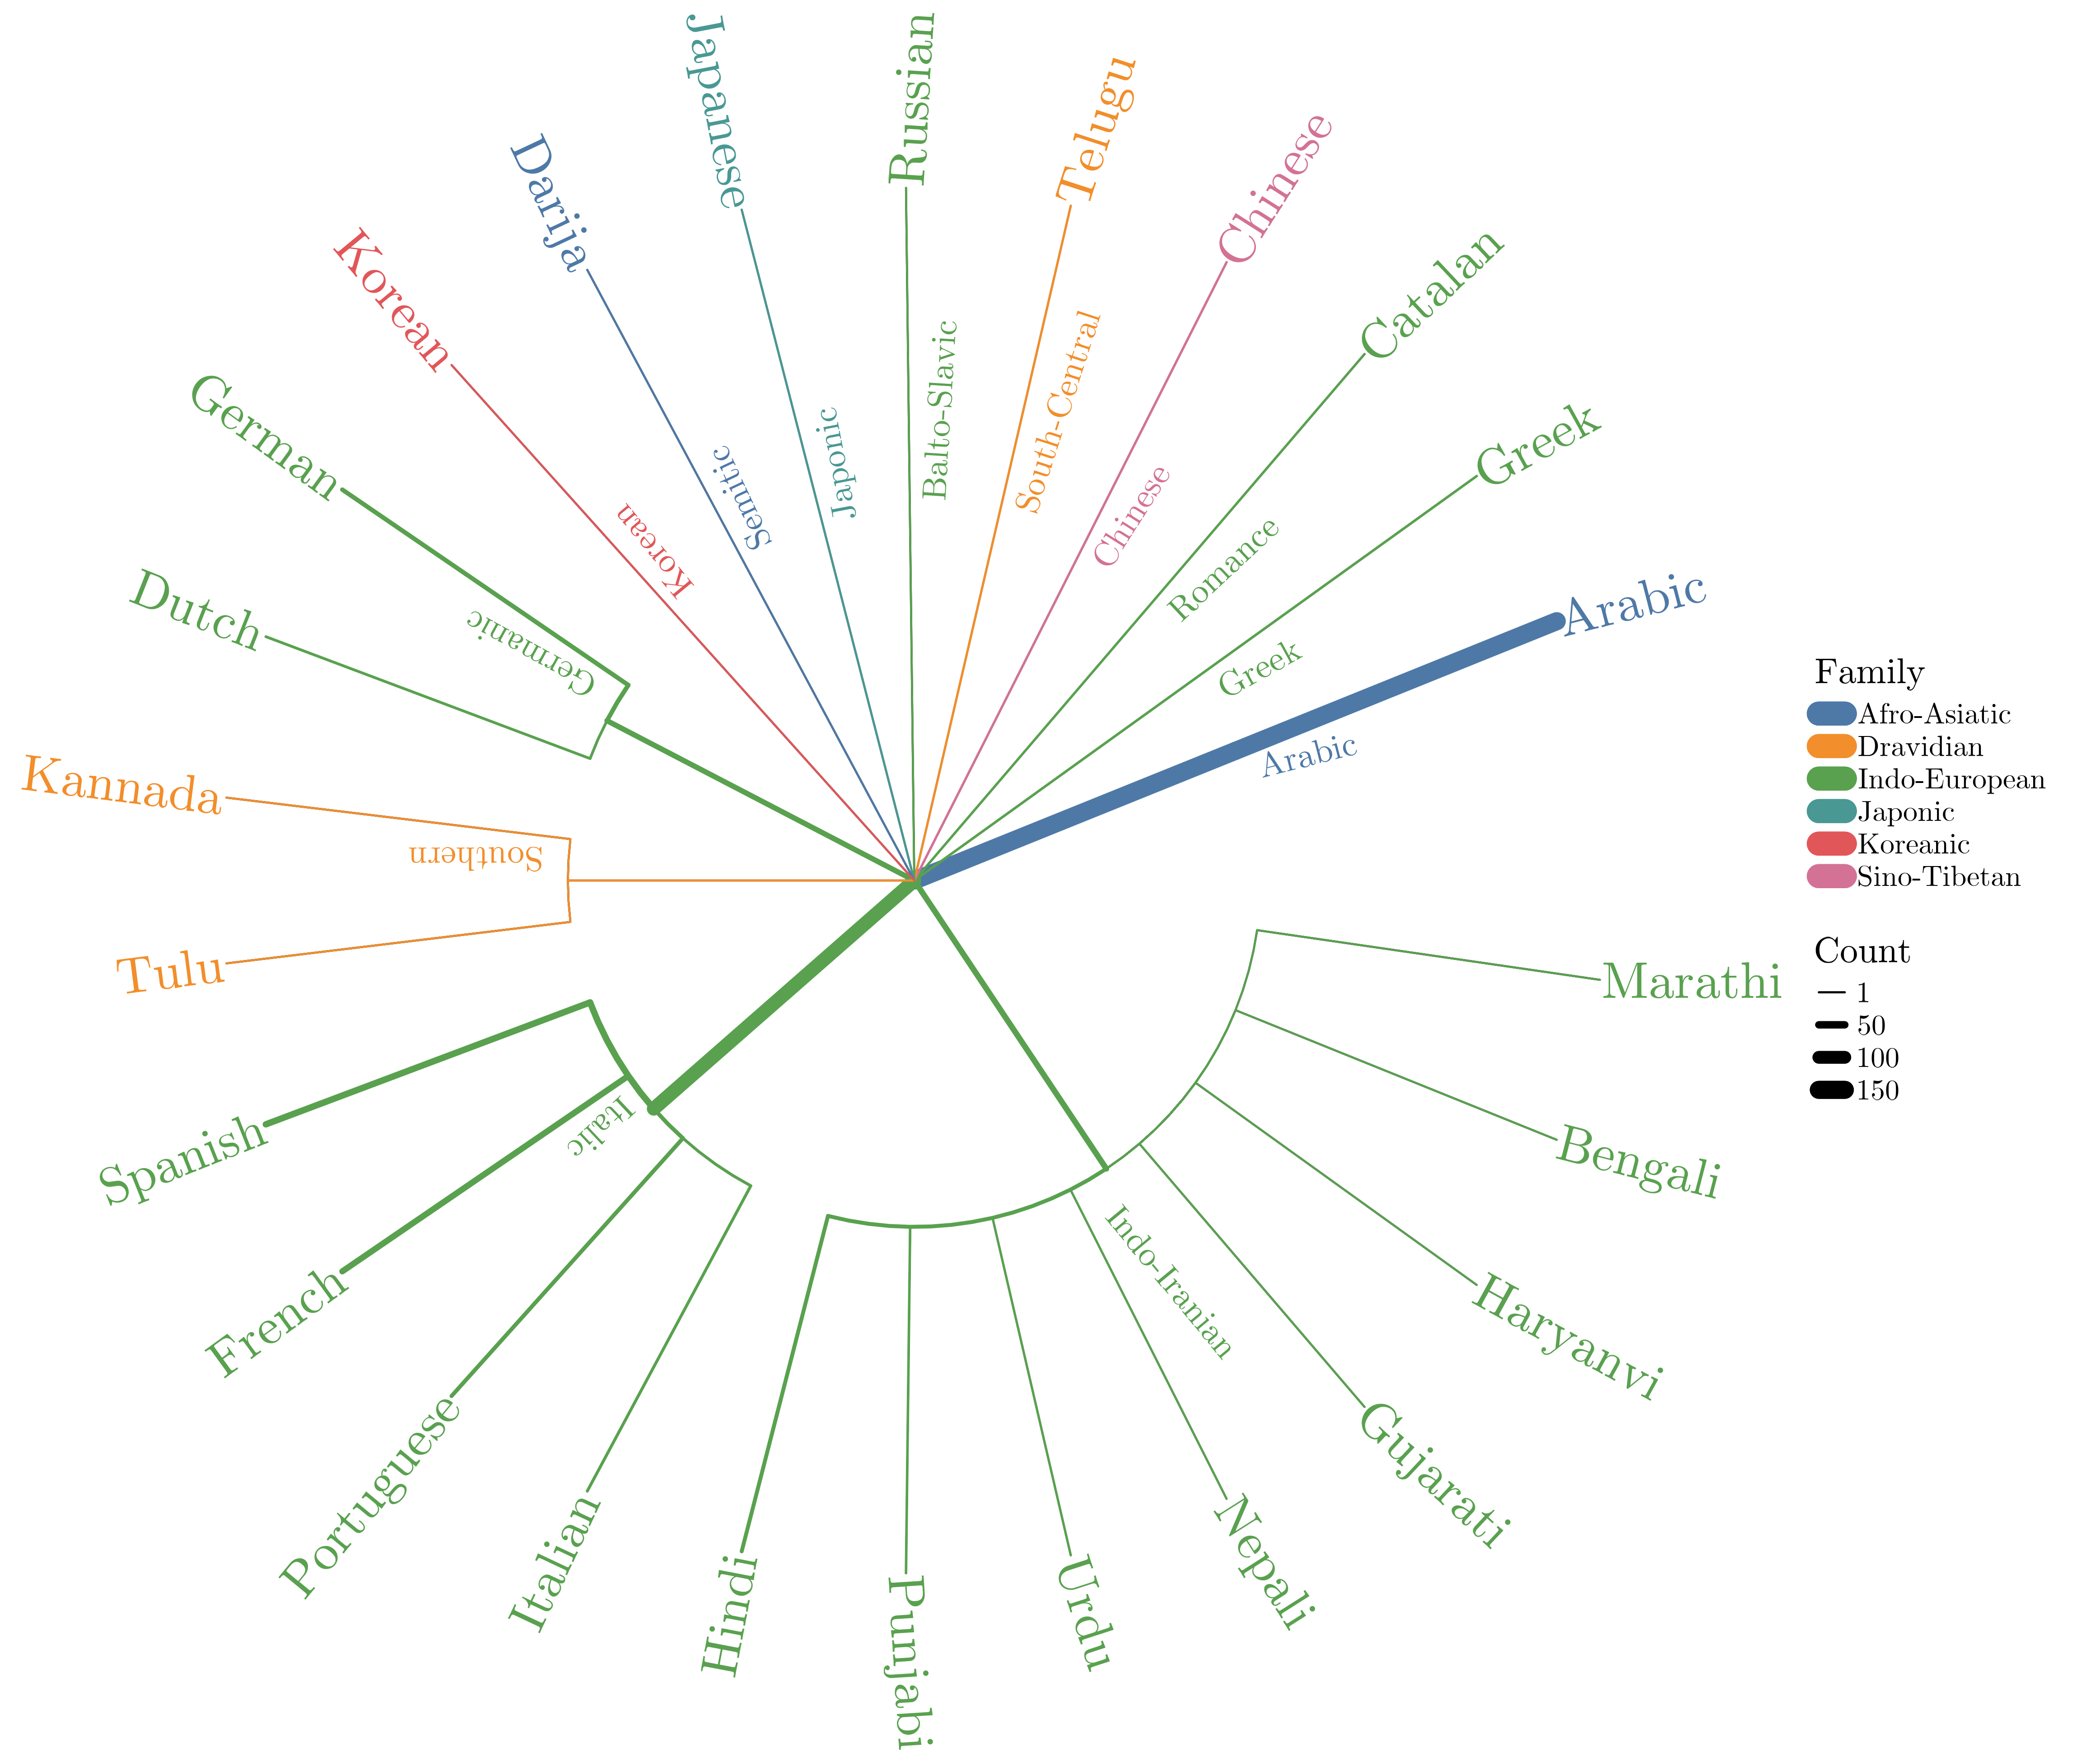
\includegraphics[width=0.52\textwidth]{Figures/exp3_languages.png}
    \end{center}
    \caption[]{\justifying Tree plot showcasing the range of language backgrounds of participants in experiment 3. The colours indicate the different language families. The inner ring holds the various branches of those families, each of those ending in individual language on the outer ring. Line thickness indicates the density of each element.}
    \label{exp3_BLPtree}
\end{figure}

% PCA
\begin{figure}[!htbp]
    \begin{center}
        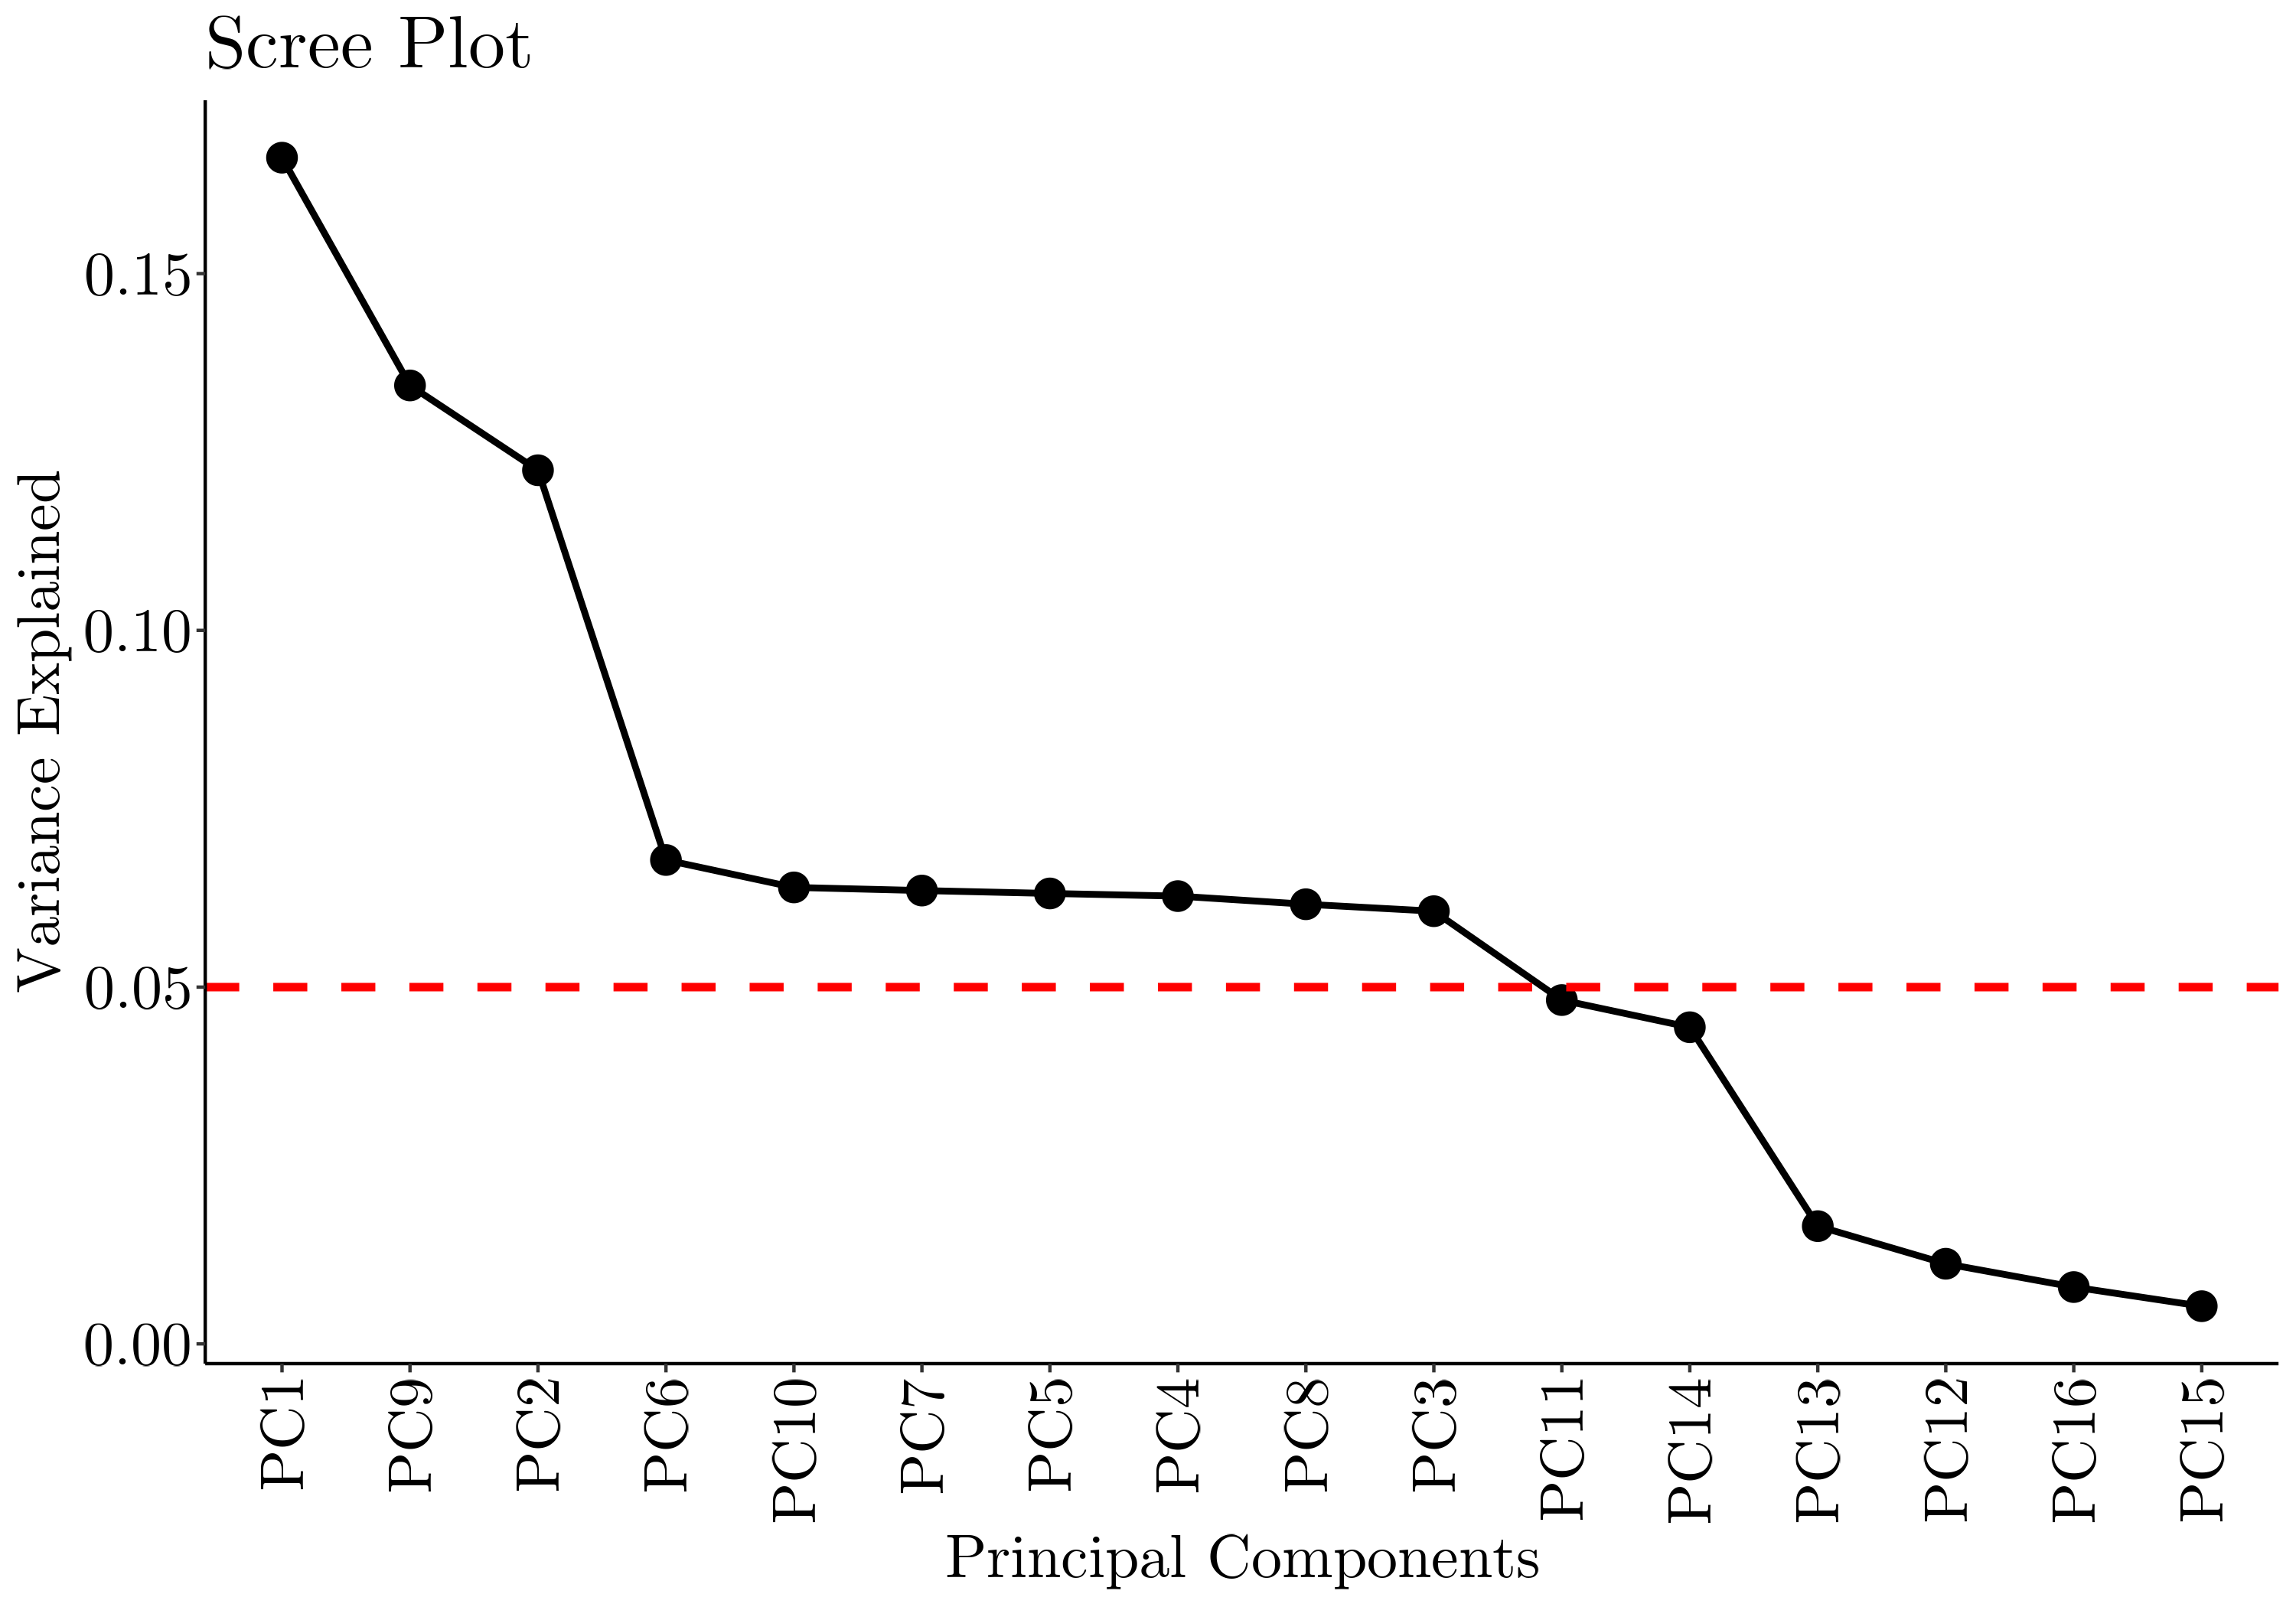
\includegraphics[width=0.6\textwidth]{Figures/Exp1_BLP_screeplt.png}
    \end{center}
    \caption[]{\justifying Scree plot of the PCA run on data for experiment 1. The red dashed line at 5\% indicates the minimum variance explained by a component for it to be considered for analysis.}
    \label{exp1_screeplot}
\end{figure}

\begin{figure}[!htbp]
    \begin{center}
        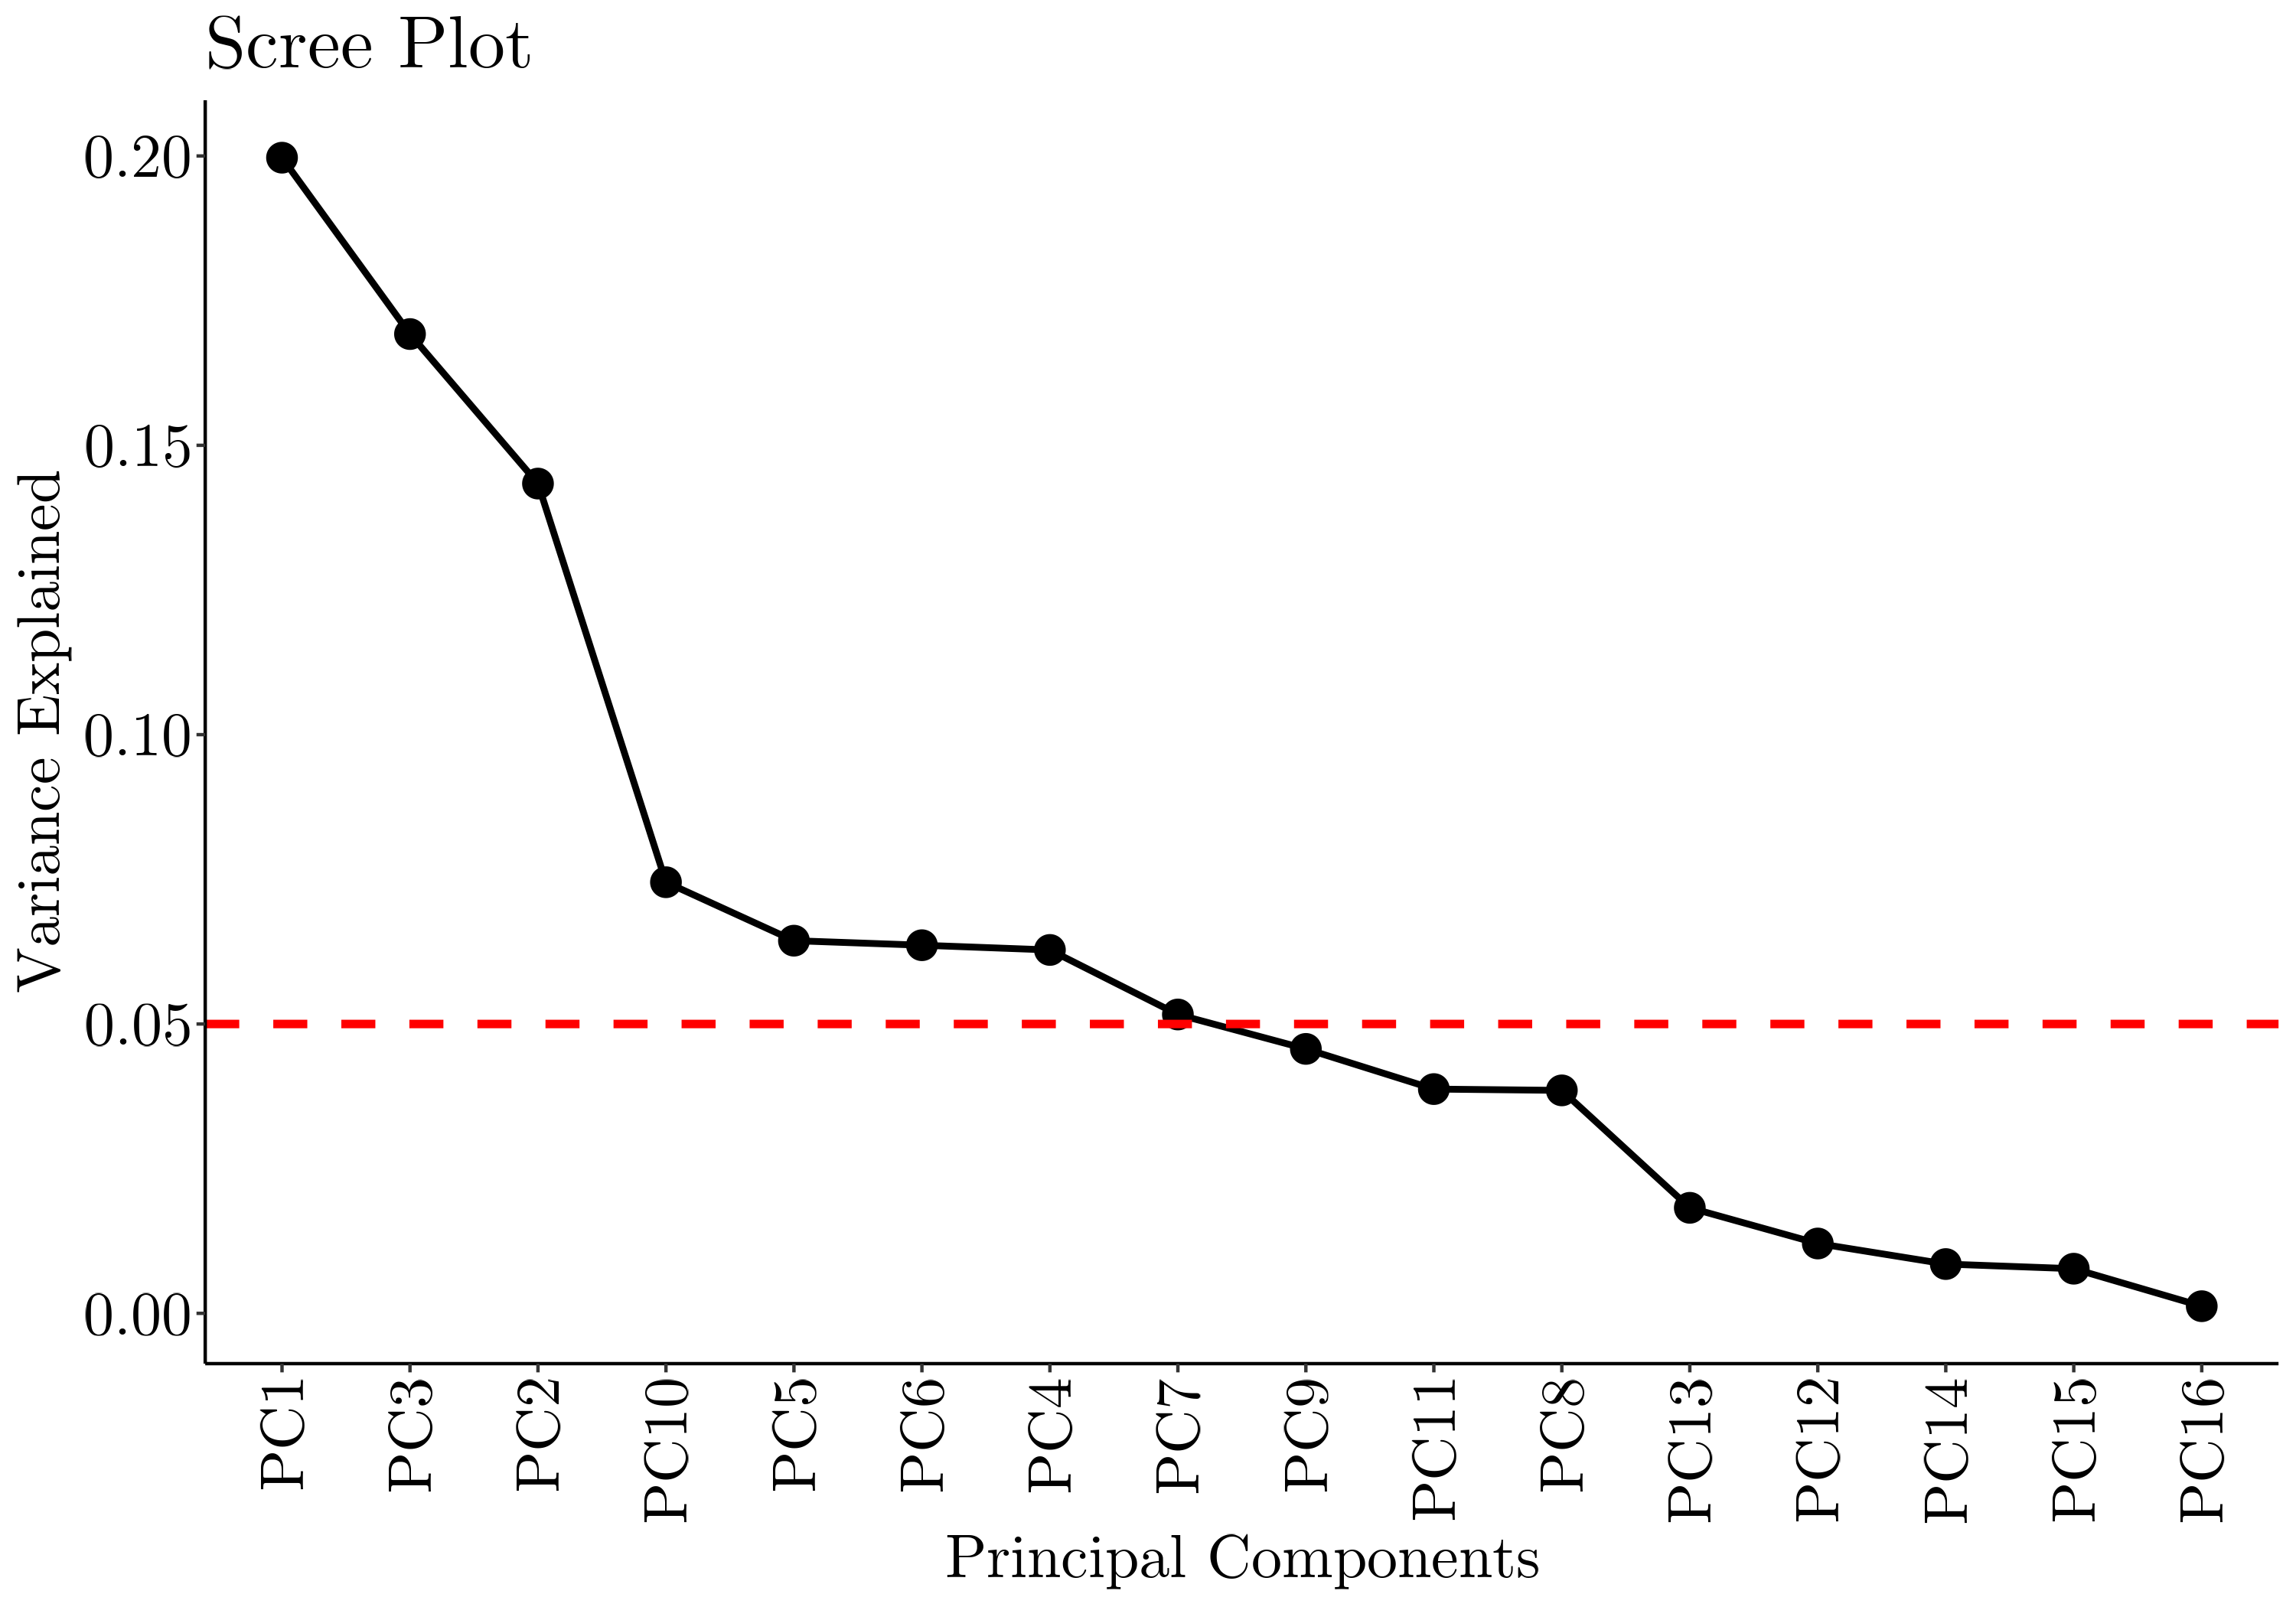
\includegraphics[width=0.6\textwidth]{Figures/exp2_BLP_screeplt.png}
    \end{center}
    \caption[]{\justifying Scree plot of the PCA run on data for experiment 2. The red dashed line at 5\% indicates the minimum variance explained by a component for it to be considered for analysis.}
    \label{exp2_screeplot}
\end{figure}

\begin{figure}[!htbp]
    \begin{center}
        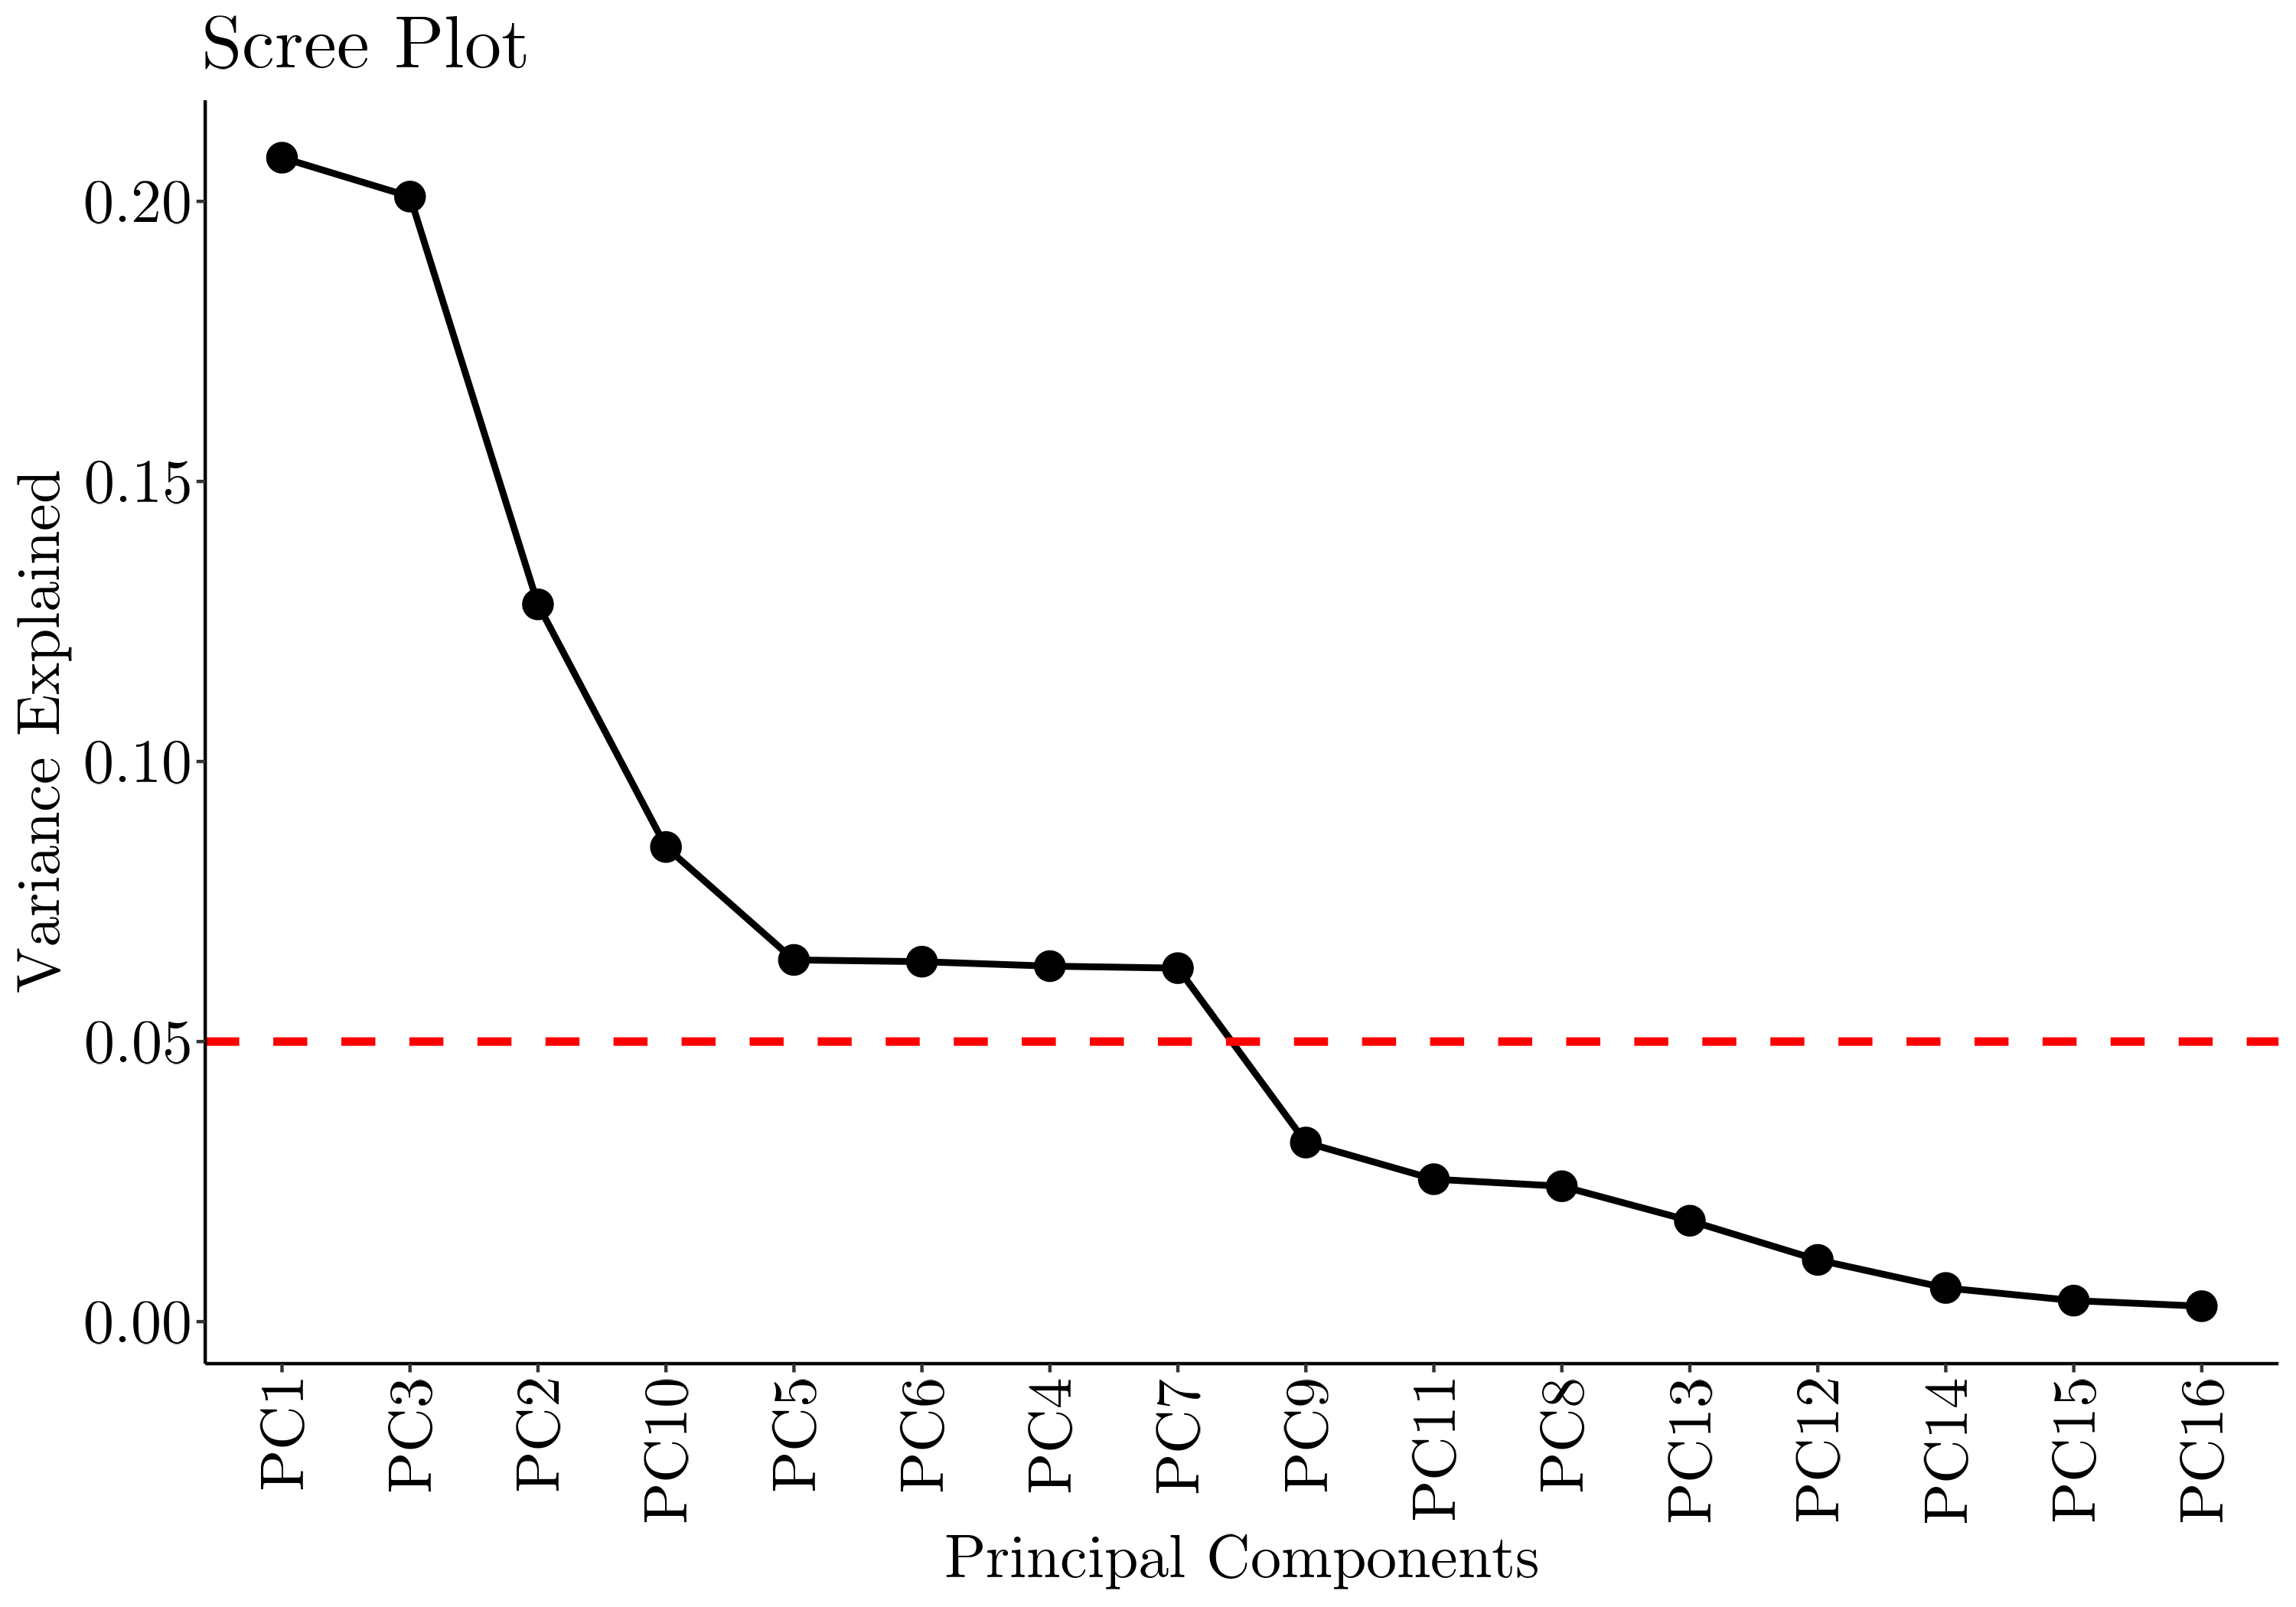
\includegraphics[width=0.6\textwidth]{Figures/exp3_BLP_screeplt.png}
    \end{center}
    \caption[]{\justifying Scree plot of the PCA run on data for experiment 3. The red dashed line at 5\% indicates the minimum variance explained by a component for it to be considered for analysis.}
    \label{exp3_screeplot}
\end{figure}




% FAMILIARITY - GENDER
\begin{table}[htbp!]
\centering
% latex table generated in R 4.5.2 by xtable 1.8-4 package
% Thu Nov 27 12:11:07 2025
\begin{tabularx}{\linewidth}{{@{} >{\RaggedRight}X*{5}{c}@{}}}
   \midrule
\multicolumn{5}{c}{\textbf{Exp. 1 Familiarity - Gender}} \\ 
  \multicolumn{5}{C{15cm}}{correct$\sim$scale(trialn)+Gender+(1\textbar sbj_ID)} \\ 
   \midrule
\textbf{Fixed effects} & $\boldsymbol\beta$ & \textbf{SE} & \textbf{z-value} & \textbf{p-value} \\ 
   \midrule
(Intercept) & 0.27 & 0.04 & 6.95 & 3.7e-12  (***) \\ 
  scale(trialn) & -0.06 & 0.03 & -2.04 & 0.042  (*) \\ 
  Other & 0.48 & 0.25 & 1.91 & 0.057  (.) \\ 
  Woman & -0.01 & 0.06 & -0.22 & 0.82  \\ 
   \midrule
\end{tabularx}


% FAMILIARITY - AGE
\input{analysis_tables/Exp. 1 Familiarity - Age}

% FAMILIARITY - PC1
\input{analysis_tables/Exp. 1 Familiarity - PC1 (L3)}

% FAMILIARITY - PC9
\input{analysis_tables/Exp. 1 Familiarity - PC9 (L4)}

% FAMILIARITY - PC2
\input{analysis_tables/Exp. 1 Familiarity - PC2 (L1 vs L2 Use)}

% FAMILIARITY - PC8
\input{analysis_tables/Exp. 1 Familiarity - PC8 (L2 History)}
\end{table}

% FAMILIARITY - PC3
\begin{table}[htbp!]
\centering
\input{analysis_tables/Exp. 1 Familiarity - PC3 (L2 Proficiency)}

% FAMILIARITY - MULTIEXP
\input{analysis_tables/Exp. 1 Familiarity - Multilingual experience}

% FAMILIARITY - L1L2DIFF
% latex table generated in R 4.5.2 by xtable 1.8-4 package
% Fri Mar 20 13:09:35 2026
\begin{tabularx}{\linewidth}{{@{} >{\RaggedRight}X*{5}{c}@{}}}
   \midrule
\multicolumn{5}{c}{\textbf{Exp. 1 Familiarity - Bilingual balance (L1-L2 difference)}} \\ 
  \multicolumn{5}{C{15cm}}{correct$\sim$scale(trialn)+scale(L1_L2_diff)+(1\textbar sbj_ID)} \\ 
   \midrule
\textbf{Fixed effects} & $\boldsymbol\beta$ & \textbf{SE} & \textbf{z-value} & \textbf{p-value} \\ 
   \midrule
(Intercept) & 0.27 & 0.03 & 9.11 & 8.3e-20  (***) \\ 
  scale(trialn) & -0.06 & 0.03 & -2.04 & 0.042  (*) \\ 
  scale(L1-L2 difference) & -0.03 & 0.03 & -0.92 & 0.36  \\ 
   \midrule
\end{tabularx}


% FAMILIARITY - ENTROPY
\input{analysis_tables/Exp. 1 Familiarity - Multilingual balance (entropy)}

% FAMILIARITY - COSSIM
\input{analysis_tables/Exp. 1 Familiarity - Multilingual balance (cosine similarity)}

% FAMILIARITY - SCRIPT
\input{analysis_tables/Exp. 1 Familiarity - Script}
\end{table}

% FAMILIARITY - CATEGORY
\begin{table}[ht]
\centering
\input{analysis_tables/Exp. 1 Familiarity - Category}
\end{table}

% YES - TESTING CONDITIONS
\begin{table}[ht]
\centering
\input{analysis_tables/Exp. 1 `Yes' responses - Conditions}

% YES - GENDER
\input{analysis_tables/Exp. 1 `Yes' responses - Gender}

% YES - AGE
\input{analysis_tables/Exp. 1 `Yes' responses - Age}
\end{table}

% YES - PC1
\begin{table}[htbp!]
\centering
% latex table generated in R 4.5.2 by xtable 1.8-4 package
% Thu Nov 27 12:03:28 2025
\begin{tabularx}{\linewidth}{{@{} >{\RaggedRight}X*{5}{c}@{}}}
   \midrule
\multicolumn{5}{c}{\textbf{Exp. 1 `Yes' responses - PC1 (L3)}} \\ 
  \multicolumn{5}{C{15cm}}{participant response$\sim$scale(trialn)+testing_condition*RC1_L3+(1\textbar sbj_ID)} \\ 
   \midrule
\textbf{Fixed effects} & $\boldsymbol\beta$ & \textbf{SE} & \textbf{z-value} & \textbf{p-value} \\ 
   \midrule
(Intercept) & -0.05 & 0.04 & -1.2 & 0.23  \\ 
  scale(trialn) & -0.08 & 0.01 & -5.18 & 2.3e-07  (***) \\ 
  1M & 0.27 & 0.04 & 7.83 & 4.9e-15  (***) \\ 
  2M & 0.67 & 0.04 & 18.41 & 1.2e-75  (***) \\ 
  PC1_L3 & 0.06 & 0.04 & 1.44 & 0.15  \\ 
  1M*PC1_L3 & -0.03 & 0.04 & -0.95 & 0.34  \\ 
  2M*PC1_L3 & -0.05 & 0.04 & -1.31 & 0.19  \\ 
   \midrule
\end{tabularx}


% YES - PC9
% latex table generated in R 4.5.2 by xtable 1.8-4 package
% Thu Nov 27 12:04:25 2025
\begin{tabularx}{\linewidth}{{@{} >{\RaggedRight}X*{5}{c}@{}}}
   \midrule
\multicolumn{5}{c}{\textbf{Exp. 1 `Yes' responses - PC9 (L4)}} \\ 
  \multicolumn{5}{C{15cm}}{participant response$\sim$testing_condition*RC9_L4+(1+testing_condition\textbar sbj_ID)} \\ 
   \midrule
\textbf{Random effects} & \textbf{Variance} & \textbf{SD} & \textbf{Corr} &  \\ 
   \midrule
(Intercept) & 0.27 & 0.52 &  &  \\ 
  1M & 0.04 & 0.2 & -0.18 &  \\ 
  2M & 0.26 & 0.51 & -0.4 & 0.97 \\ 
   \midrule
\textbf{Fixed effects} & $\boldsymbol\beta$ & \textbf{SE} & \textbf{z-value} & \textbf{p-value} \\ 
   \midrule
(Intercept) & -0.05 & 0.04 & -1.07 & 0.29  \\ 
  1M & 0.28 & 0.04 & 7.23 & 4.9e-13  (***) \\ 
  2M & 0.67 & 0.05 & 12.77 & 2.5e-37  (***) \\ 
  PC9_L4 & -0.06 & 0.05 & -1.33 & 0.18  \\ 
  1M*PC9_L4 & 0.03 & 0.04 & 0.78 & 0.44  \\ 
  2M*PC9_L4 & 0.03 & 0.05 & 0.61 & 0.54  \\ 
   \midrule
\end{tabularx}


% YES - PC2
\input{analysis_tables/Exp. 1 `Yes' responses - PC2 (L1 vs L2 Use)}
\end{table}

% YES - PC8
\begin{table}[htbp!]
\centering
\input{analysis_tables/Exp. 1 `Yes' responses - PC8 (L2 History)}

% YES - PC3
\input{analysis_tables/Exp. 1 `Yes' responses - PC3 (L2 Proficiency)}

% YES - MULTILINGUAL EXPERIENCE
\input{analysis_tables/Exp. 1 `Yes' responses - Multilingual experience}
\end{table}

% YES - L1-L2 DIFFERENCE
\begin{table}[htbp!]
\centering
% latex table generated in R 4.5.2 by xtable 1.8-4 package
% Tue Dec 16 09:02:03 2025
\begin{tabularx}{\linewidth}{{@{} >{\RaggedRight}X*{5}{c}@{}}}
   \midrule
\multicolumn{5}{c}{\textbf{Exp. 1 `Yes' responses - Bilingual balance (L1-L2 difference)}} \\ 
  \multicolumn{5}{C{15cm}}{observed$\sim$testing_condition*scale(L1_L2_diff)+(1\textbar sbj_ID)} \\ 
   \midrule
\textbf{Fixed effects} & $\boldsymbol\beta$ & \textbf{SE} & \textbf{z-value} & \textbf{p-value} \\ 
   \midrule
(Intercept) & -0.05 & 0.04 & -1.24 & 0.22  \\ 
  1M & 0.29 & 0.04 & 8.17 & 3.2e-16  (***) \\ 
  2M & 0.69 & 0.04 & 18.75 & 2.1e-78  (***) \\ 
  scale(L1-L2 difference) & -0.01 & 0.04 & -0.31 & 0.76  \\ 
  1M*scale(L1-L2 difference) & -0.06 & 0.04 & -1.83 & 0.07  (.) \\ 
  2M*scale(L1-L2 difference) & -0.08 & 0.04 & -2.21 & 0.03  (*) \\ 
   \midrule
\end{tabularx}


% YES - ENTROPY
\input{analysis_tables/Exp. 1 `Yes' responses - Multilingual balance (Entropy)}

% YES - COSINE SIMILARITY
\input{analysis_tables/Exp. 1 `Yes' responses - Multilingual balance (cosine similarity)}

% YES - SCRIPT
\input{analysis_tables/Exp. 1 `Yes' responses - Script}
\end{table}

% YES - CATEGORY
\begin{table}[htbp!]
\centering
\input{analysis_tables/Exp. 1 `Yes' responses - Category}
\end{table}

% 2M
\begin{table}[htbp!]
\centering
% latex table generated in R 4.5.2 by xtable 1.8-4 package
% Thu Nov 27 12:09:53 2025
\begin{tabularx}{\linewidth}{{@{} >{\RaggedRight}X*{5}{c}@{}}}
   \midrule
\multicolumn{5}{c}{\textbf{Exp. 1 2M}} \\ 
  \multicolumn{5}{C{15cm}}{participant response$\sim$scale(trialn)+string nature+(1\textbar sbj_ID)} \\ 
   \midrule
\textbf{Fixed effects} & $\boldsymbol\beta$ & \textbf{SE} & \textbf{z-value} & \textbf{p-value} \\ 
   \midrule
(Intercept) & 0.62 & 0.06 & 11.24 & 2.6e-29  (***) \\ 
  scale(trialn) & -0.16 & 0.03 & -5.61 & 2.1e-08  (***) \\ 
  within_language & -0.01 & 0.05 & -0.23 & 0.82  \\ 
   \midrule
\end{tabularx}


% 2M - GENDER
% latex table generated in R 4.5.2 by xtable 1.8-4 package
% Thu Nov 27 12:10:03 2025
\begin{tabularx}{\linewidth}{{@{} >{\RaggedRight}X*{5}{c}@{}}}
   \midrule
\multicolumn{5}{c}{\textbf{Exp. 1 2M - Gender}} \\ 
  \multicolumn{5}{C{15cm}}{participant response$\sim$scale(trialn)+string nature*Gender+(1+string nature\textbar sbj_ID)} \\ 
   \midrule
\textbf{Random effects} &  & \textbf{Variance} & \textbf{SD} & \textbf{Corr} \\ 
   \midrule
 & (Intercept) & 0.34 & 0.58 &  \\ 
   & within_language & 0.01 & 0.1 & -1 \\ 
   \midrule
\textbf{Fixed effects} & $\boldsymbol\beta$ & \textbf{SE} & \textbf{z-value} & \textbf{p-value} \\ 
   \midrule
(Intercept) & 0.6 & 0.08 & 7.85 & 4.1e-15  (***) \\ 
  scale(trialn) & -0.16 & 0.03 & -5.6 & 2.2e-08  (***) \\ 
  within_language &  6.2e-04 & 0.07 &  8.5e-03 & 0.99  \\ 
  Other & 0.51 & 0.48 & 1.07 & 0.29  \\ 
  Woman & 0.06 & 0.12 & 0.53 & 0.59  \\ 
  within_language*Other & 0.58 & 0.52 & 1.11 & 0.27  \\ 
  within_language*Woman & -0.08 & 0.11 & -0.68 & 0.5  \\ 
   \midrule
\end{tabularx}


% 2M - AGE
% latex table generated in R 4.5.2 by xtable 1.8-4 package
% Thu Nov 27 12:10:06 2025
\begin{tabularx}{\linewidth}{{@{} >{\RaggedRight}X*{5}{c}@{}}}
   \midrule
\multicolumn{5}{c}{\textbf{Exp. 1 2M - Age}} \\ 
  \multicolumn{5}{C{15cm}}{participant response$\sim$scale(trialn)+string nature*scale(Age)+(1\textbar sbj_ID)} \\ 
   \midrule
\textbf{Fixed effects} & $\boldsymbol\beta$ & \textbf{SE} & \textbf{z-value} & \textbf{p-value} \\ 
   \midrule
(Intercept) & 0.62 & 0.06 & 11.27 & 1.8e-29  (***) \\ 
  scale(trialn) & -0.16 & 0.03 & -5.63 & 1.8e-08  (***) \\ 
  within_language & -0.01 & 0.05 & -0.23 & 0.82  \\ 
  scale(Age) & 0.03 & 0.06 & 0.52 & 0.6  \\ 
  within_language*scale(Age) & 0.04 & 0.06 & 0.74 & 0.46  \\ 
   \midrule
\end{tabularx}


% 2M - PC1
% latex table generated in R 4.5.2 by xtable 1.8-4 package
% Thu Nov 27 12:10:08 2025
\begin{tabularx}{\linewidth}{{@{} >{\RaggedRight}X*{5}{c}@{}}}
   \midrule
\multicolumn{5}{c}{\textbf{Exp. 1 2M - PC1 (L3)}} \\ 
  \multicolumn{5}{C{15cm}}{participant response$\sim$scale(trialn)+string nature*RC1_L3+(1\textbar sbj_ID)} \\ 
   \midrule
\textbf{Fixed effects} & $\boldsymbol\beta$ & \textbf{SE} & \textbf{z-value} & \textbf{p-value} \\ 
   \midrule
(Intercept) & 0.62 & 0.06 & 11.24 & 2.5e-29  (***) \\ 
  scale(trialn) & -0.16 & 0.03 & -5.6 & 2.1e-08  (***) \\ 
  within_language & -0.01 & 0.06 & -0.23 & 0.82  \\ 
  PC1_L3 & 0.02 & 0.06 & 0.32 & 0.75  \\ 
  within_language*PC1_L3 &  3.3e-04 & 0.06 &  6.0e-03 & 1  \\ 
   \midrule
\end{tabularx}

\end{table}

% 2M - PC9
\begin{table}[htbp!]
\centering
\input{analysis_tables/Exp. 1 2M - PC9 (L4)}

% 2M - PC2
% latex table generated in R 4.5.2 by xtable 1.8-4 package
% Thu Nov 27 12:10:13 2025
\begin{tabularx}{\linewidth}{{@{} >{\RaggedRight}X*{5}{c}@{}}}
   \midrule
\multicolumn{5}{c}{\textbf{Exp. 1 2M - PC2 (L1 vs L2 Use)}} \\ 
  \multicolumn{5}{C{15cm}}{participant response$\sim$scale(trialn)+string nature*RC2_use_L1vsL2+(1\textbar sbj_ID)} \\ 
   \midrule
\textbf{Fixed effects} & $\boldsymbol\beta$ & \textbf{SE} & \textbf{z-value} & \textbf{p-value} \\ 
   \midrule
(Intercept) & 0.62 & 0.06 & 11.27 & 1.9e-29  (***) \\ 
  scale(trialn) & -0.16 & 0.03 & -5.61 & 2.0e-08  (***) \\ 
  within_language & -0.01 & 0.05 & -0.22 & 0.82  \\ 
  PC2_L1vsL2_Use & 0.07 & 0.06 & 1.21 & 0.23  \\ 
  within_language*PC2_L1vsL2_Use &  3.5e-04 & 0.06 &  6.3e-03 & 0.99  \\ 
   \midrule
\end{tabularx}


% 2M - PC8
% latex table generated in R 4.5.2 by xtable 1.8-4 package
% Thu Nov 27 12:10:15 2025
\begin{tabularx}{\linewidth}{{@{} >{\RaggedRight}X*{5}{c}@{}}}
   \midrule
\multicolumn{5}{c}{\textbf{Exp. 1 2M - PC8 (L2 History)}} \\ 
  \multicolumn{5}{C{15cm}}{participant response$\sim$scale(trialn)+string nature*RC8_hist_L2+(1\textbar sbj_ID)} \\ 
   \midrule
\textbf{Fixed effects} & $\boldsymbol\beta$ & \textbf{SE} & \textbf{z-value} & \textbf{p-value} \\ 
   \midrule
(Intercept) & 0.62 & 0.06 & 11.32 & 1.0e-29  (***) \\ 
  scale(trialn) & -0.16 & 0.03 & -5.62 & 1.9e-08  (***) \\ 
  within_language & -0.01 & 0.06 & -0.22 & 0.82  \\ 
  PC8_L2_History & 0.11 & 0.06 & 1.91 & 0.056  (.) \\ 
  within_language*PC8_L2_History & -1.6e-03 & 0.06 & -0.03 & 0.98  \\ 
   \midrule
\end{tabularx}


% 2M - PC3
% latex table generated in R 4.5.2 by xtable 1.8-4 package
% Thu Nov 27 12:10:18 2025
\begin{tabularx}{\linewidth}{{@{} >{\RaggedRight}X*{5}{c}@{}}}
   \midrule
\multicolumn{5}{c}{\textbf{Exp. 1 2M - PC3 (L2 Proficiency)}} \\ 
  \multicolumn{5}{C{15cm}}{participant response$\sim$scale(trialn)+string nature*RC3_prof_L2+(1\textbar sbj_ID)} \\ 
   \midrule
\textbf{Fixed effects} & $\boldsymbol\beta$ & \textbf{SE} & \textbf{z-value} & \textbf{p-value} \\ 
   \midrule
(Intercept) & 0.63 & 0.06 & 11.32 & 1.0e-29  (***) \\ 
  scale(trialn) & -0.16 & 0.03 & -5.57 & 2.6e-08  (***) \\ 
  within_language & -0.01 & 0.06 & -0.27 & 0.79  \\ 
  PC3_L2_Proficiency & 0.13 & 0.05 & 2.34 & 0.02  (*) \\ 
  within_language*PC3_L2_Proficiency & -0.1 & 0.05 & -1.89 & 0.058  (.) \\ 
   \midrule
\end{tabularx}


% 2M - MULTILINGUAL EXPERIENCE
% latex table generated in R 4.5.2 by xtable 1.8-4 package
% Thu Nov 27 12:10:39 2025
\begin{tabularx}{\linewidth}{{@{} >{\RaggedRight}X*{5}{c}@{}}}
   \midrule
\multicolumn{5}{c}{\textbf{Exp. 1 2M - Multilingual experience}} \\ 
  \multicolumn{5}{C{15cm}}{participant response$\sim$scale(trialn)+string nature*scale(multiexp)+(1\textbar sbj_ID)} \\ 
   \midrule
\textbf{Fixed effects} & $\boldsymbol\beta$ & \textbf{SE} & \textbf{z-value} & \textbf{p-value} \\ 
   \midrule
(Intercept) & 0.62 & 0.06 & 11.29 & 1.5e-29  (***) \\ 
  scale(trialn) & -0.16 & 0.03 & -5.61 & 2.0e-08  (***) \\ 
  within_language & -0.01 & 0.06 & -0.22 & 0.82  \\ 
  scale(Multilingual experience) & 0.06 & 0.06 & 1.16 & 0.25  \\ 
  within_language*scale(Multilingual experience) & 0.03 & 0.06 & 0.47 & 0.64  \\ 
   \midrule
\end{tabularx}

\end{table}

% 2M - L1-L2 DIFFERENCE
\begin{table}[htbp!]
\centering
% latex table generated in R 4.5.2 by xtable 1.8-4 package
% Tue Dec 16 09:02:51 2025
\begin{tabularx}{\linewidth}{{@{} >{\RaggedRight}X*{5}{c}@{}}}
   \midrule
\multicolumn{5}{c}{\textbf{Exp. 1 2M - Bilingual Balance (L1-L2 difference)}} \\ 
  \multicolumn{5}{C{15cm}}{observed$\sim$scale(trialn)+expected*scale(L1_L2_diff)+(1\textbar sbj_ID)} \\ 
   \midrule
\textbf{Fixed effects} & $\boldsymbol\beta$ & \textbf{SE} & \textbf{z-value} & \textbf{p-value} \\ 
   \midrule
(Intercept) & 0.64 & 0.05 & 11.73 & 9.3e-32  (***) \\ 
  scale(trialn) & -0.15 & 0.03 & -5.27 & 1.4e-07  (***) \\ 
  within_language & -0.02 & 0.06 & -0.31 & 0.76  \\ 
  scale(L1-L2 difference) & -0.08 & 0.05 & -1.43 & 0.15  \\ 
  within_language*scale(L1-L2 difference) & -0.02 & 0.06 & -0.37 & 0.71  \\ 
   \midrule
\end{tabularx}


% 2M - ENTROPY
% latex table generated in R 4.5.2 by xtable 1.8-4 package
% Thu Nov 27 12:10:31 2025
\begin{tabularx}{\linewidth}{{@{} >{\RaggedRight}X*{5}{c}@{}}}
   \midrule
\multicolumn{5}{c}{\textbf{Exp. 1 2M - Multilingual balance (Entropy)}} \\ 
  \multicolumn{5}{C{15cm}}{participant response$\sim$scale(trialn)+string nature*ent+(1+string nature\textbar sbj_ID)} \\ 
   \midrule
\textbf{Random effects} &  & \textbf{Variance} & \textbf{SD} & \textbf{Corr} \\ 
   \midrule
 & (Intercept) & 0.33 & 0.58 &  \\ 
   & within_language & 0.01 & 0.09 & -1 \\ 
   \midrule
\textbf{Fixed effects} & $\boldsymbol\beta$ & \textbf{SE} & \textbf{z-value} & \textbf{p-value} \\ 
   \midrule
(Intercept) & 0.42 & 0.18 & 2.29 & 0.02  (*) \\ 
  scale(trialn) & -0.16 & 0.03 & -5.62 & 2.0e-08  (***) \\ 
  within_language & -0.08 & 0.17 & -0.46 & 0.64  \\ 
  Entropy & 0.16 & 0.14 & 1.22 & 0.22  \\ 
  within_language*Entropy & 0.04 & 0.13 & 0.35 & 0.73  \\ 
   \midrule
\end{tabularx}


% 2M - COSSIM
% latex table generated in R 4.5.2 by xtable 1.8-4 package
% Thu Nov 27 12:10:44 2025
\begin{tabularx}{\linewidth}{{@{} >{\RaggedRight}X*{5}{c}@{}}}
   \midrule
\multicolumn{5}{c}{\textbf{Exp. 1 2M - Multilingual balance (cosine similarity)}} \\ 
  \multicolumn{5}{C{15cm}}{participant response$\sim$scale(trialn)+string nature*scale(cossim)+(1\textbar sbj_ID)} \\ 
   \midrule
\textbf{Fixed effects} & $\boldsymbol\beta$ & \textbf{SE} & \textbf{z-value} & \textbf{p-value} \\ 
   \midrule
(Intercept) & 0.62 & 0.06 & 11.24 & 2.5e-29  (***) \\ 
  scale(trialn) & -0.16 & 0.03 & -5.61 & 2.0e-08  (***) \\ 
  within_language & -0.01 & 0.05 & -0.22 & 0.83  \\ 
  scale(Cosine similarity) &  3.3e-03 & 0.06 & 0.06 & 0.95  \\ 
  within_language*scale(Cosine similarity) & 0.04 & 0.05 & 0.64 & 0.52  \\ 
   \midrule
\end{tabularx}


% 2M - SCRIPT
% latex table generated in R 4.5.2 by xtable 1.8-4 package
% Thu Nov 27 12:10:49 2025
\begin{tabularx}{\linewidth}{{@{} >{\RaggedRight}X*{5}{c}@{}}}
   \midrule
\multicolumn{5}{c}{\textbf{Exp. 1 2M - Script}} \\ 
  \multicolumn{5}{C{15cm}}{participant response$\sim$scale(trialn)+string nature*script+(1\textbar sbj_ID)} \\ 
   \midrule
\textbf{Fixed effects} & $\boldsymbol\beta$ & \textbf{SE} & \textbf{z-value} & \textbf{p-value} \\ 
   \midrule
(Intercept) & 0.6 & 0.06 & 10.31 & 6.4e-25  (***) \\ 
  scale(trialn) & -0.16 & 0.03 & -5.59 & 2.2e-08  (***) \\ 
  within_language & -2.3e-03 & 0.06 & -0.04 & 0.97  \\ 
  Different script & 0.2 & 0.18 & 1.08 & 0.28  \\ 
  within_language*Different script & -0.1 & 0.18 & -0.54 & 0.59  \\ 
   \midrule
\end{tabularx}

\end{table}

% 2M - CATEGORY
\begin{table}[htbp!]
\centering
% latex table generated in R 4.5.2 by xtable 1.8-4 package
% Thu Nov 27 12:11:05 2025
\begin{tabularx}{\linewidth}{{@{} >{\RaggedRight}X*{5}{c}@{}}}
   \midrule
\multicolumn{5}{c}{\textbf{Exp. 1 2M - Category}} \\ 
  \multicolumn{5}{C{15cm}}{participant response$\sim$string nature*category+(1\textbar sbj_ID)} \\ 
   \midrule
\textbf{Fixed effects} & $\boldsymbol\beta$ & \textbf{SE} & \textbf{z-value} & \textbf{p-value} \\ 
   \midrule
(Intercept) & -0.27 & 0.37 & -0.74 & 0.46  \\ 
  within_language & 0.23 & 0.36 & 0.64 & 0.52  \\ 
  Bilingual & 0.93 & 0.38 & 2.46 & 0.01  (*) \\ 
  Trilingual & 0.91 & 0.38 & 2.38 & 0.02  (*) \\ 
  Quadrilingual & 0.89 & 0.38 & 2.31 & 0.02  (*) \\ 
  within_language*Bilingual & -0.28 & 0.37 & -0.74 & 0.46  \\ 
  within_language*Trilingual & -0.29 & 0.38 & -0.76 & 0.45  \\ 
  within_language*Quadrilingual & -0.16 & 0.38 & -0.41 & 0.68  \\ 
   \midrule
\end{tabularx}

\end{table}














% FAMILIARITY - GENDER
\begin{table}[htbp!]
\centering
\input{analysis_tables/Exp. 2 Familiarity - Gender}

% FAMILIARITY - AGE
\input{analysis_tables/Exp. 2 Familiarity - Age}

% FAMILIARITY - PC1
\input{analysis_tables/Exp. 2 Familiarity - PC1 (L4)}

% FAMILIARITY - PC3
% latex table generated in R 4.6.0 by xtable 1.8-8 package
% Wed Jul  1 18:48:51 2026
\begin{tabularx}{\linewidth}{{@{} >{\RaggedRight}X*{5}{c}@{}}}
   \midrule
\multicolumn{5}{c}{\textbf{Exp. 2 Familiarity - PC3 (L3)}} \\ 
  \multicolumn{5}{C{15cm}}{correct$\sim$scale(trialn)+RC3_L3+(1\textbar sbj_ID)} \\ 
   \midrule
\textbf{Fixed effects} & $\boldsymbol\beta$ & \textbf{SE} & \textbf{z-value} & \textbf{p-value} \\ 
   \midrule
(Intercept) & 0.3 & 0.03 & 10.13 & 4.1e-24  (***) \\ 
  scale(trialn) & -0.09 & 0.03 & -3.12 & 1.8e-03  (**) \\ 
  PC3_L3 & -0.04 & 0.03 & -1.3 & 0.19  \\ 
   \midrule
\end{tabularx}


% FAMILIARITY - PC2
\input{analysis_tables/Exp. 2 Familiarity - PC2 (L1 vs L2 Use)}

% FAMILIARITY - PC7
\input{analysis_tables/Exp. 2 Familiarity - PC7 (L2 History)}
\end{table}

% FAMILIARITY - PC9
\begin{table}[htbp!]
\centering
\input{analysis_tables/Exp. 2 Familiarity - PC9 (L4 Use)}

% FAMILIARITY - MULTIEXP
% latex table generated in R 4.6.0 by xtable 1.8-8 package
% Wed Jul  1 18:49:19 2026
\begin{tabularx}{\linewidth}{{@{} >{\RaggedRight}X*{5}{c}@{}}}
   \midrule
\multicolumn{5}{c}{\textbf{Exp. 2 Familiarity - Multilingual experience}} \\ 
  \multicolumn{5}{C{15cm}}{correct$\sim$scale(trialn)+scale(multiexp)+(1\textbar sbj_ID)} \\ 
   \midrule
\textbf{Fixed effects} & $\boldsymbol\beta$ & \textbf{SE} & \textbf{z-value} & \textbf{p-value} \\ 
   \midrule
(Intercept) & 0.3 & 0.03 & 10.12 & 4.5e-24  (***) \\ 
  scale(trialn) & -0.09 & 0.03 & -3.12 & 1.8e-03  (**) \\ 
  scale(Multilingual experience) & -0.03 & 0.03 & -1.15 & 0.25  \\ 
   \midrule
\end{tabularx}


% FAMILIARITY - L1L2DIFF
% latex table generated in R 4.5.2 by xtable 1.8-4 package
% Tue Dec 16 09:08:48 2025
\begin{tabularx}{\linewidth}{{@{} >{\RaggedRight}X*{5}{c}@{}}}
   \midrule
\multicolumn{5}{c}{\textbf{Exp. 2 Familiarity - Bilingual balance (L1-L2 difference)}} \\ 
  \multicolumn{5}{C{15cm}}{correct$\sim$scale(trialn)+scale(L1_L2_diff)+(1\textbar sbj_ID)} \\ 
   \midrule
\textbf{Fixed effects} & $\boldsymbol\beta$ & \textbf{SE} & \textbf{z-value} & \textbf{p-value} \\ 
   \midrule
(Intercept) & 0.29 & 0.03 & 9.35 & 8.8e-21  (***) \\ 
  scale(trialn) & -0.09 & 0.03 & -3.24 & 1.2e-03  (**) \\ 
  scale(L1-L2 difference) & -0.01 & 0.03 & -0.44 & 0.66  \\ 
   \midrule
\end{tabularx}


% FAMILIARITY - ENTROPY
% latex table generated in R 4.6.0 by xtable 1.8-8 package
% Wed Jul  1 18:49:10 2026
\begin{tabularx}{\linewidth}{{@{} >{\RaggedRight}X*{5}{c}@{}}}
   \midrule
\multicolumn{5}{c}{\textbf{Exp. 2 Familiarity - Multilingual balance (entropy)}} \\ 
  \multicolumn{5}{C{15cm}}{correct$\sim$scale(trialn)+ent+(1\textbar sbj_ID)} \\ 
   \midrule
\textbf{Fixed effects} & $\boldsymbol\beta$ & \textbf{SE} & \textbf{z-value} & \textbf{p-value} \\ 
   \midrule
(Intercept) & 0.41 & 0.07 & 5.89 & 3.9e-09  (***) \\ 
  scale(trialn) & -0.09 & 0.03 & -3.12 & 1.8e-03  (**) \\ 
  Entropy & -0.09 & 0.05 & -1.71 & 0.09  (.) \\ 
   \midrule
\end{tabularx}


% FAMILIARITY - COSSIM
\input{analysis_tables/Exp. 2 Familiarity - Multilingual balance (cosine similarity)}

% FAMILIARITY - SCRIPT
% latex table generated in R 4.6.0 by xtable 1.8-8 package
% Wed Jul  1 18:49:38 2026
\begin{tabularx}{\linewidth}{{@{} >{\RaggedRight}X*{5}{c}@{}}}
   \midrule
\multicolumn{5}{c}{\textbf{Exp. 2 Familiarity - Script}} \\ 
  \multicolumn{5}{C{15cm}}{correct$\sim$scale(trialn)+script+(1\textbar sbj_ID)} \\ 
   \midrule
\textbf{Fixed effects} & $\boldsymbol\beta$ & \textbf{SE} & \textbf{z-value} & \textbf{p-value} \\ 
   \midrule
(Intercept) & 0.32 & 0.03 & 9.84 & 7.9e-23  (***) \\ 
  scale(trialn) & -0.09 & 0.03 & -3.12 & 1.8e-03  (**) \\ 
  Different script & -0.11 & 0.08 & -1.33 & 0.18  \\ 
   \midrule
\end{tabularx}

\end{table}

% FAMILIARITY - CATEGORY
\begin{table}[ht]
\centering
\input{analysis_tables/Exp. 2 Familiarity - Category}
\end{table}

% YES - TESTING CONDITIONS
\begin{table}[ht]
\centering
% latex table generated in R 4.6.0 by xtable 1.8-8 package
% Wed Jul  1 18:13:28 2026
\begin{tabularx}{\linewidth}{{@{} >{\RaggedRight}X*{5}{c}@{}}}
   \midrule
\multicolumn{5}{c}{\textbf{Exp. 2 `Yes' responses - Conditions}} \\ 
  \multicolumn{5}{C{15cm}}{participant response$\sim$scale(trialn)+testing_condition+(1+testing_condition\textbar sbj_ID)} \\ 
   \midrule
\textbf{Random effects} & \textbf{Variance} & \textbf{SD} & \textbf{Corr} &  \\ 
   \midrule
(Intercept) & 0.37 & 0.61 &  &  \\ 
  1M & 0.1 & 0.32 & -0.61 &  \\ 
  2M & 0.22 & 0.46 & -0.46 & 0.95 \\ 
   \midrule
\textbf{Fixed effects} & $\boldsymbol\beta$ & \textbf{SE} & \textbf{z-value} & \textbf{p-value} \\ 
   \midrule
(Intercept) & 0.09 & 0.05 & 1.75 & 0.08  (.) \\ 
  scale(trialn) & -0.08 & 0.01 & -5.56 & 2.7e-08  (***) \\ 
  1M & 0.25 & 0.04 & 5.84 & 5.1e-09  (***) \\ 
  2M & 0.55 & 0.05 & 10.85 & 2.0e-27  (***) \\ 
   \midrule
\end{tabularx}


% YES - GENDER
% latex table generated in R 4.6.0 by xtable 1.8-8 package
% Wed Jul  1 18:14:32 2026
\begin{tabularx}{\linewidth}{{@{} >{\RaggedRight}X*{5}{c}@{}}}
   \midrule
\multicolumn{5}{c}{\textbf{Exp. 2 `Yes' responses - Gender}} \\ 
  \multicolumn{5}{C{15cm}}{participant response$\sim$scale(trialn)+testing_condition*Gender+(1+testing_condition\textbar sbj_ID)} \\ 
   \midrule
\textbf{Random effects} & \textbf{Variance} & \textbf{SD} & \textbf{Corr} &  \\ 
   \midrule
(Intercept) & 0.37 & 0.61 &  &  \\ 
  1M & 0.1 & 0.31 & -0.63 &  \\ 
  2M & 0.21 & 0.46 & -0.47 & 0.96 \\ 
   \midrule
\textbf{Fixed effects} & $\boldsymbol\beta$ & \textbf{SE} & \textbf{z-value} & \textbf{p-value} \\ 
   \midrule
(Intercept) & 0.08 & 0.07 & 1.05 & 0.29  \\ 
  scale(trialn) & -0.08 & 0.01 & -5.52 & 3.4e-08  (***) \\ 
  1M & 0.17 & 0.06 & 2.82 & 4.9e-03  (**) \\ 
  2M & 0.49 & 0.07 & 6.98 & 2.9e-12  (***) \\ 
  Woman & 0.03 & 0.1 & 0.27 & 0.78  \\ 
  1M*Woman & 0.17 & 0.09 & 1.99 & 0.047  (*) \\ 
  2M*Woman & 0.11 & 0.1 & 1.14 & 0.25  \\ 
   \midrule
\end{tabularx}


% YES - AGE
% latex table generated in R 4.6.0 by xtable 1.8-8 package
% Wed Jul  1 18:15:16 2026
\begin{tabularx}{\linewidth}{{@{} >{\RaggedRight}X*{5}{c}@{}}}
   \midrule
\multicolumn{5}{c}{\textbf{Exp. 2 `Yes' responses - Age}} \\ 
  \multicolumn{5}{C{15cm}}{participant response$\sim$scale(trialn)+testing_condition*scale(Age)+(1+testing_condition\textbar sbj_ID)} \\ 
   \midrule
\textbf{Random effects} & \textbf{Variance} & \textbf{SD} & \textbf{Corr} &  \\ 
   \midrule
(Intercept) & 0.37 & 0.61 &  &  \\ 
  1M & 0.1 & 0.31 & -0.62 &  \\ 
  2M & 0.2 & 0.45 & -0.47 & 0.95 \\ 
   \midrule
\textbf{Fixed effects} & $\boldsymbol\beta$ & \textbf{SE} & \textbf{z-value} & \textbf{p-value} \\ 
   \midrule
(Intercept) & 0.09 & 0.05 & 1.74 & 0.08  (.) \\ 
  scale(trialn) & -0.08 & 0.01 & -5.56 & 2.7e-08  (***) \\ 
  1M & 0.25 & 0.04 & 5.89 & 3.8e-09  (***) \\ 
  2M & 0.55 & 0.05 & 10.99 & 4.1e-28  (***) \\ 
  scale(Age) &  2.6e-03 & 0.05 & 0.05 & 0.96  \\ 
  1M*scale(Age) & 0.06 & 0.04 & 1.45 & 0.15  \\ 
  2M*scale(Age) & 0.1 & 0.05 & 2.02 & 0.043  (*) \\ 
   \midrule
\end{tabularx}

\end{table}

% YES - PC1
\begin{table}[htbp!]
\centering
% latex table generated in R 4.6.0 by xtable 1.8-8 package
% Wed Jul  1 18:16:00 2026
\begin{tabularx}{\linewidth}{{@{} >{\RaggedRight}X*{5}{c}@{}}}
   \midrule
\multicolumn{5}{c}{\textbf{Exp. 2 `Yes' responses - PC1 (L4)}} \\ 
  \multicolumn{5}{C{15cm}}{participant response$\sim$scale(trialn)+testing_condition*RC1_L4+(1+testing_condition\textbar sbj_ID)} \\ 
   \midrule
\textbf{Random effects} & \textbf{Variance} & \textbf{SD} & \textbf{Corr} &  \\ 
   \midrule
(Intercept) & 0.36 & 0.6 &  &  \\ 
  1M & 0.1 & 0.32 & -0.6 &  \\ 
  2M & 0.21 & 0.46 & -0.45 & 0.95 \\ 
   \midrule
\textbf{Fixed effects} & $\boldsymbol\beta$ & \textbf{SE} & \textbf{z-value} & \textbf{p-value} \\ 
   \midrule
(Intercept) & 0.09 & 0.05 & 1.76 & 0.08  (.) \\ 
  scale(trialn) & -0.08 & 0.01 & -5.56 & 2.7e-08  (***) \\ 
  1M & 0.25 & 0.04 & 5.85 & 5.0e-09  (***) \\ 
  2M & 0.55 & 0.05 & 10.87 & 1.6e-27  (***) \\ 
  PC1_L4 & 0.09 & 0.05 & 1.79 & 0.07  (.) \\ 
  1M*PC1_L4 & -0.03 & 0.04 & -0.67 & 0.5  \\ 
  2M*PC1_L4 & -0.05 & 0.05 & -1.01 & 0.31  \\ 
   \midrule
\end{tabularx}


% YES - PC3
% latex table generated in R 4.6.0 by xtable 1.8-8 package
% Wed Jul  1 18:16:57 2026
\begin{tabularx}{\linewidth}{{@{} >{\RaggedRight}X*{5}{c}@{}}}
   \midrule
\multicolumn{5}{c}{\textbf{Exp. 2 `Yes' responses - PC3 (L3)}} \\ 
  \multicolumn{5}{C{15cm}}{participant response$\sim$scale(trialn)+testing_condition*RC3_L3+(1+testing_condition\textbar sbj_ID)} \\ 
   \midrule
\textbf{Random effects} & \textbf{Variance} & \textbf{SD} & \textbf{Corr} &  \\ 
   \midrule
(Intercept) & 0.37 & 0.61 &  &  \\ 
  1M & 0.1 & 0.31 & -0.6 &  \\ 
  2M & 0.22 & 0.46 & -0.46 & 0.97 \\ 
   \midrule
\textbf{Fixed effects} & $\boldsymbol\beta$ & \textbf{SE} & \textbf{z-value} & \textbf{p-value} \\ 
   \midrule
(Intercept) & 0.09 & 0.05 & 1.76 & 0.08  (.) \\ 
  scale(trialn) & -0.08 & 0.01 & -5.55 & 2.8e-08  (***) \\ 
  1M & 0.25 & 0.04 & 5.87 & 4.5e-09  (***) \\ 
  2M & 0.55 & 0.05 & 10.85 & 2.0e-27  (***) \\ 
  PC3_L3 & 0.06 & 0.05 & 1.15 & 0.25  \\ 
  1M*PC3_L3 & -0.07 & 0.04 & -1.74 & 0.08  (.) \\ 
  2M*PC3_L3 & -0.02 & 0.05 & -0.35 & 0.72  \\ 
   \midrule
\end{tabularx}

\end{table}

% YES - PC2
\begin{table}[htbp!]
\centering
% latex table generated in R 4.6.0 by xtable 1.8-8 package
% Wed Jul  1 18:18:11 2026
\begin{tabularx}{\linewidth}{{@{} >{\RaggedRight}X*{5}{c}@{}}}
   \midrule
\multicolumn{5}{c}{\textbf{Exp. 2 `Yes' responses - PC2 (L1 vs L2 Use)}} \\ 
  \multicolumn{5}{C{15cm}}{participant response$\sim$scale(trialn)+testing_condition*RC2_use_L1vsL2+(1+testing_condition\textbar sbj_ID)} \\ 
   \midrule
\textbf{Random effects} & \textbf{Variance} & \textbf{SD} & \textbf{Corr} &  \\ 
   \midrule
(Intercept) & 0.37 & 0.61 &  &  \\ 
  1M & 0.1 & 0.32 & -0.62 &  \\ 
  2M & 0.21 & 0.45 & -0.48 & 0.95 \\ 
   \midrule
\textbf{Fixed effects} & $\boldsymbol\beta$ & \textbf{SE} & \textbf{z-value} & \textbf{p-value} \\ 
   \midrule
(Intercept) & 0.09 & 0.05 & 1.74 & 0.08  (.) \\ 
  scale(trialn) & -0.08 & 0.01 & -5.54 & 3.0e-08  (***) \\ 
  1M & 0.25 & 0.04 & 5.86 & 4.6e-09  (***) \\ 
  2M & 0.55 & 0.05 & 10.95 & 6.5e-28  (***) \\ 
  PC2_L1vsL2_Use &  9.9e-03 & 0.05 & 0.19 & 0.85  \\ 
  1M*PC2_L1vsL2_Use & 0.06 & 0.04 & 1.33 & 0.18  \\ 
  2M*PC2_L1vsL2_Use & 0.1 & 0.05 & 2.03 & 0.042  (*) \\ 
   \midrule
\end{tabularx}


% YES - PC7
\input{analysis_tables/Exp. 2 `Yes' responses - PC7 (L2 History)}
\end{table}

% YES - PC9
\begin{table}[htbp!]
\centering
% latex table generated in R 4.6.0 by xtable 1.8-8 package
% Wed Jul  1 18:22:22 2026
\begin{tabularx}{\linewidth}{{@{} >{\RaggedRight}X*{5}{c}@{}}}
   \midrule
\multicolumn{5}{c}{\textbf{Exp. 2 `Yes' responses - PC9 (L4 Use)}} \\ 
  \multicolumn{5}{C{15cm}}{participant response$\sim$scale(trialn)+testing_condition*RC9_use_L4+(1+testing_condition\textbar sbj_ID)} \\ 
   \midrule
\textbf{Random effects} & \textbf{Variance} & \textbf{SD} & \textbf{Corr} &  \\ 
   \midrule
(Intercept) & 0.37 & 0.61 &  &  \\ 
  1M & 0.1 & 0.32 & -0.61 &  \\ 
  2M & 0.22 & 0.46 & -0.46 & 0.96 \\ 
   \midrule
\textbf{Fixed effects} & $\boldsymbol\beta$ & \textbf{SE} & \textbf{z-value} & \textbf{p-value} \\ 
   \midrule
(Intercept) & 0.09 & 0.05 & 1.75 & 0.08  (.) \\ 
  scale(trialn) & -0.08 & 0.01 & -5.56 & 2.7e-08  (***) \\ 
  1M & 0.25 & 0.04 & 5.81 & 6.3e-09  (***) \\ 
  2M & 0.55 & 0.05 & 10.86 & 1.8e-27  (***) \\ 
  PC9_L4_Use & -0.01 & 0.05 & -0.24 & 0.81  \\ 
  1M*PC9_L4_Use & -0.03 & 0.05 & -0.56 & 0.58  \\ 
  2M*PC9_L4_Use & 0.02 & 0.06 & 0.34 & 0.74  \\ 
   \midrule
\end{tabularx}


% YES - MULTILINGUAL EXPERIENCE
\input{analysis_tables/Exp. 2 `Yes' responses - Multilingual experience}

% YES - L1-L2 DIFFERENCE
% latex table generated in R 4.5.2 by xtable 1.8-4 package
% Tue Dec 16 09:07:51 2025
\begin{tabularx}{\linewidth}{{@{} >{\RaggedRight}X*{5}{c}@{}}}
   \midrule
\multicolumn{5}{c}{\textbf{Exp. 2 `Yes' responses - Bilingual balance (L1-L2 difference)}} \\ 
  \multicolumn{5}{C{15cm}}{participant response$\sim$scale(trialn)+testing_condition*scale(L1_L2_diff)+(1\textbar sbj_ID)} \\ 
   \midrule
\textbf{Fixed effects} & $\boldsymbol\beta$ & \textbf{SE} & \textbf{z-value} & \textbf{p-value} \\ 
   \midrule
(Intercept) & 0.09 & 0.05 & 1.82 & 0.07  (.) \\ 
  scale(trialn) & -0.09 & 0.02 & -5.4 & 6.7e-08  (***) \\ 
  1M & 0.24 & 0.04 & 6.4 & 1.5e-10  (***) \\ 
  2M & 0.57 & 0.04 & 14.7 & 6.6e-49  (***) \\ 
  scale(L1-L2 difference) & -0.13 & 0.05 & -2.79 & 5.3e-03  (**) \\ 
  1M*scale(L1-L2 difference) & -6.9e-03 & 0.04 & -0.18 & 0.85  \\ 
  2M*scale(L1-L2 difference) & -0.04 & 0.04 & -0.97 & 0.33  \\ 
   \midrule
\end{tabularx}

\end{table}

% YES - ENTROPY
\begin{table}[htbp!]
\centering
\input{analysis_tables/Exp. 2 `Yes' responses - Multilingual balance (Entropy)}

% YES - COSINE SIMILARITY
% latex table generated in R 4.6.0 by xtable 1.8-8 package
% Wed Jul  1 18:37:15 2026
\begin{tabularx}{\linewidth}{{@{} >{\RaggedRight}X*{5}{c}@{}}}
   \midrule
\multicolumn{5}{c}{\textbf{Exp. 2 `Yes' responses - Multilingual balance (cosine similarity)}} \\ 
  \multicolumn{5}{C{15cm}}{participant response$\sim$testing_condition*cossim+(1\textbar sbj_ID)} \\ 
   \midrule
\textbf{Fixed effects} & $\boldsymbol\beta$ & \textbf{SE} & \textbf{z-value} & \textbf{p-value} \\ 
   \midrule
(Intercept) & -1.38 & 1.15 & -1.2 & 0.23  \\ 
  1M & -1.39 & 0.89 & -1.56 & 0.12  \\ 
  2M & -0.07 & 0.9 & -0.08 & 0.94  \\ 
  Cosine similarity & 1.53 & 1.19 & 1.28 & 0.2  \\ 
  1M*Cosine similarity & 1.72 & 0.93 & 1.85 & 0.06  (.) \\ 
  2M*Cosine similarity & 0.64 & 0.94 & 0.69 & 0.49  \\ 
   \midrule
\end{tabularx}


% YES - SCRIPT
\input{analysis_tables/Exp. 2 `Yes' responses - Script}
\end{table}

% YES - CATEGORY
\begin{table}[htbp!]
\centering
\input{analysis_tables/Exp. 2 `Yes' responses - Category}
\end{table}

% 2M
\begin{table}[htbp!]
\centering
% latex table generated in R 4.5.2 by xtable 1.8-4 package
% Thu Nov 27 11:24:26 2025
\begin{tabularx}{\linewidth}{{@{} >{\RaggedRight}X*{5}{c}@{}}}
   \midrule
\multicolumn{5}{c}{\textbf{Exp. 2 2M}} \\ 
  \multicolumn{5}{C{15cm}}{participant response$\sim$scale(trialn)+string nature+(1+string nature\textbar sbj_ID)} \\ 
   \midrule
\textbf{Random effects} &  & \textbf{Variance} & \textbf{SD} & \textbf{Corr} \\ 
   \midrule
 & (Intercept) & 0.36 & 0.6 &  \\ 
   & within_language & 0.01 & 0.09 & -0.64 \\ 
   \midrule
\textbf{Fixed effects} & $\boldsymbol\beta$ & \textbf{SE} & \textbf{z-value} & \textbf{p-value} \\ 
   \midrule
(Intercept) & 0.66 & 0.06 & 11.19 & 4.8e-29  (***) \\ 
  scale(trialn) & -0.11 & 0.03 & -4.24 & 2.2e-05  (***) \\ 
  within_language & -0.06 & 0.05 & -1.07 & 0.29  \\ 
   \midrule
\end{tabularx}


% 2M - GENDER
% latex table generated in R 4.5.2 by xtable 1.8-4 package
% Thu Nov 27 11:24:35 2025
\begin{tabularx}{\linewidth}{{@{} >{\RaggedRight}X*{5}{c}@{}}}
   \midrule
\multicolumn{5}{c}{\textbf{Exp. 2 2M - Gender}} \\ 
  \multicolumn{5}{C{15cm}}{participant response$\sim$scale(trialn)+string nature*Gender+(1+string nature\textbar sbj_ID)} \\ 
   \midrule
\textbf{Random effects} &  & \textbf{Variance} & \textbf{SD} & \textbf{Corr} \\ 
   \midrule
 & (Intercept) & 0.36 & 0.6 &  \\ 
   & within_language & 0.01 & 0.09 & -0.66 \\ 
   \midrule
\textbf{Fixed effects} & $\boldsymbol\beta$ & \textbf{SE} & \textbf{z-value} & \textbf{p-value} \\ 
   \midrule
(Intercept) & 0.6 & 0.08 & 7.32 & 2.5e-13  (***) \\ 
  scale(trialn) & -0.11 & 0.03 & -4.24 & 2.3e-05  (***) \\ 
  within_language & -0.07 & 0.07 & -0.95 & 0.34  \\ 
  Woman & 0.12 & 0.12 & 1.02 & 0.31  \\ 
  within_language*Woman & 0.03 & 0.11 & 0.25 & 0.81  \\ 
   \midrule
\end{tabularx}


% 2M - AGE
% latex table generated in R 4.5.2 by xtable 1.8-4 package
% Thu Nov 27 11:24:45 2025
\begin{tabularx}{\linewidth}{{@{} >{\RaggedRight}X*{5}{c}@{}}}
   \midrule
\multicolumn{5}{c}{\textbf{Exp. 2 2M - Age}} \\ 
  \multicolumn{5}{C{15cm}}{participant response$\sim$scale(trialn)+string nature*scale(Age)+(1+string nature\textbar sbj_ID)} \\ 
   \midrule
\textbf{Random effects} &  & \textbf{Variance} & \textbf{SD} & \textbf{Corr} \\ 
   \midrule
 & (Intercept) & 0.35 & 0.59 &  \\ 
   & within_language & 0.01 & 0.09 & -0.67 \\ 
   \midrule
\textbf{Fixed effects} & $\boldsymbol\beta$ & \textbf{SE} & \textbf{z-value} & \textbf{p-value} \\ 
   \midrule
(Intercept) & 0.66 & 0.06 & 11.26 & 2.2e-29  (***) \\ 
  scale(trialn) & -0.11 & 0.03 & -4.24 & 2.2e-05  (***) \\ 
  within_language & -0.06 & 0.05 & -1.07 & 0.28  \\ 
  scale(Age) & 0.1 & 0.06 & 1.68 & 0.09  (.) \\ 
  within_language*scale(Age) &  4.9e-03 & 0.05 & 0.09 & 0.93  \\ 
   \midrule
\end{tabularx}


% 2M - PC1
% latex table generated in R 4.5.2 by xtable 1.8-4 package
% Thu Nov 27 11:24:54 2025
\begin{tabularx}{\linewidth}{{@{} >{\RaggedRight}X*{5}{c}@{}}}
   \midrule
\multicolumn{5}{c}{\textbf{Exp. 2 2M - PC1 (L4)}} \\ 
  \multicolumn{5}{C{15cm}}{participant response$\sim$scale(trialn)+string nature*RC1_L4+(1+string nature\textbar sbj_ID)} \\ 
   \midrule
\textbf{Random effects} &  & \textbf{Variance} & \textbf{SD} & \textbf{Corr} \\ 
   \midrule
 & (Intercept) & 0.36 & 0.6 &  \\ 
   & within_language & 0.01 & 0.09 & -0.65 \\ 
   \midrule
\textbf{Fixed effects} & $\boldsymbol\beta$ & \textbf{SE} & \textbf{z-value} & \textbf{p-value} \\ 
   \midrule
(Intercept) & 0.66 & 0.06 & 11.2 & 4.0e-29  (***) \\ 
  scale(trialn) & -0.11 & 0.03 & -4.24 & 2.2e-05  (***) \\ 
  within_language & -0.06 & 0.05 & -1.07 & 0.29  \\ 
  PC1_L4 & 0.04 & 0.06 & 0.69 & 0.49  \\ 
  within_language*PC1_L4 &  1.4e-03 & 0.05 & 0.03 & 0.98  \\ 
   \midrule
\end{tabularx}

\end{table}

% 2M - PC3
\begin{table}[htbp!]
\centering
% latex table generated in R 4.5.2 by xtable 1.8-4 package
% Thu Nov 27 11:25:09 2025
\begin{tabularx}{\linewidth}{{@{} >{\RaggedRight}X*{5}{c}@{}}}
   \midrule
\multicolumn{5}{c}{\textbf{Exp. 2 2M - PC3 (L3)}} \\ 
  \multicolumn{5}{C{15cm}}{participant response$\sim$scale(trialn)+string nature*RC3_L3+(1+string nature\textbar sbj_ID)} \\ 
   \midrule
\textbf{Random effects} &  & \textbf{Variance} & \textbf{SD} & \textbf{Corr} \\ 
   \midrule
 & (Intercept) & 0.36 & 0.6 &  \\ 
   & within_language & 0.01 & 0.08 & -0.73 \\ 
   \midrule
\textbf{Fixed effects} & $\boldsymbol\beta$ & \textbf{SE} & \textbf{z-value} & \textbf{p-value} \\ 
   \midrule
(Intercept) & 0.66 & 0.06 & 11.19 & 4.6e-29  (***) \\ 
  scale(trialn) & -0.11 & 0.03 & -4.25 & 2.2e-05  (***) \\ 
  within_language & -0.06 & 0.05 & -1.06 & 0.29  \\ 
  PC3_L3 & 0.02 & 0.06 & 0.42 & 0.67  \\ 
  within_language*PC3_L3 & 0.03 & 0.05 & 0.62 & 0.54  \\ 
   \midrule
\end{tabularx}


% 2M - PC2
% latex table generated in R 4.5.2 by xtable 1.8-4 package
% Thu Nov 27 11:25:17 2025
\begin{tabularx}{\linewidth}{{@{} >{\RaggedRight}X*{5}{c}@{}}}
   \midrule
\multicolumn{5}{c}{\textbf{Exp. 2 2M - PC2 (L1 vs L2 Use)}} \\ 
  \multicolumn{5}{C{15cm}}{participant response$\sim$scale(trialn)+string nature*RC2_use_L1vsL2+(1+string nature\textbar sbj_ID)} \\ 
   \midrule
\textbf{Random effects} &  & \textbf{Variance} & \textbf{SD} & \textbf{Corr} \\ 
   \midrule
 & (Intercept) & 0.34 & 0.58 &  \\ 
   & within_language & 0.01 & 0.09 & -0.63 \\ 
   \midrule
\textbf{Fixed effects} & $\boldsymbol\beta$ & \textbf{SE} & \textbf{z-value} & \textbf{p-value} \\ 
   \midrule
(Intercept) & 0.66 & 0.06 & 11.35 & 7.7e-30  (***) \\ 
  scale(trialn) & -0.11 & 0.03 & -4.23 & 2.4e-05  (***) \\ 
  within_language & -0.06 & 0.05 & -1.06 & 0.29  \\ 
  PC2_L1vsL2_Use & 0.13 & 0.06 & 2.25 & 0.02  (*) \\ 
  within_language*PC2_L1vsL2_Use & -0.02 & 0.05 & -0.35 & 0.72  \\ 
   \midrule
\end{tabularx}


% 2M - PC7
% latex table generated in R 4.5.2 by xtable 1.8-4 package
% Thu Nov 27 11:25:28 2025
\begin{tabularx}{\linewidth}{{@{} >{\RaggedRight}X*{5}{c}@{}}}
   \midrule
\multicolumn{5}{c}{\textbf{Exp. 2 2M - PC7 (L2 History)}} \\ 
  \multicolumn{5}{C{15cm}}{participant response$\sim$scale(trialn)+string nature*RC7_hist_L2+(1+string nature\textbar sbj_ID)} \\ 
   \midrule
\textbf{Random effects} &  & \textbf{Variance} & \textbf{SD} & \textbf{Corr} \\ 
   \midrule
 & (Intercept) & 0.35 & 0.59 &  \\ 
   & within_language & 0.01 & 0.09 & -0.61 \\ 
   \midrule
\textbf{Fixed effects} & $\boldsymbol\beta$ & \textbf{SE} & \textbf{z-value} & \textbf{p-value} \\ 
   \midrule
(Intercept) & 0.66 & 0.06 & 11.33 & 9.7e-30  (***) \\ 
  scale(trialn) & -0.11 & 0.03 & -4.24 & 2.2e-05  (***) \\ 
  within_language & -0.06 & 0.05 & -1.08 & 0.28  \\ 
  PC7_L2_History & 0.11 & 0.06 & 1.87 & 0.06  (.) \\ 
  within_language*PC7_L2_History & -0.02 & 0.05 & -0.38 & 0.71  \\ 
   \midrule
\end{tabularx}

\end{table}

% 2M - PC9
\begin{table}[htbp!]
\centering
% latex table generated in R 4.5.2 by xtable 1.8-4 package
% Thu Nov 27 11:25:37 2025
\begin{tabularx}{\linewidth}{{@{} >{\RaggedRight}X*{5}{c}@{}}}
   \midrule
\multicolumn{5}{c}{\textbf{Exp. 2 2M - PC9 (L4 Use)}} \\ 
  \multicolumn{5}{C{15cm}}{participant response$\sim$scale(trialn)+string nature*RC9_use_L4+(1+string nature\textbar sbj_ID)} \\ 
   \midrule
\textbf{Random effects} &  & \textbf{Variance} & \textbf{SD} & \textbf{Corr} \\ 
   \midrule
 & (Intercept) & 0.36 & 0.6 &  \\ 
   & within_language & 0.01 & 0.09 & -0.64 \\ 
   \midrule
\textbf{Fixed effects} & $\boldsymbol\beta$ & \textbf{SE} & \textbf{z-value} & \textbf{p-value} \\ 
   \midrule
(Intercept) & 0.66 & 0.06 & 11.19 & 4.7e-29  (***) \\ 
  scale(trialn) & -0.11 & 0.03 & -4.24 & 2.3e-05  (***) \\ 
  within_language & -0.06 & 0.05 & -1.07 & 0.28  \\ 
  PC9_L4_Use & 0.01 & 0.06 & 0.18 & 0.86  \\ 
  within_language*PC9_L4_Use & -7.9e-03 & 0.06 & -0.13 & 0.9  \\ 
   \midrule
\end{tabularx}


% 2M - MULTIEXP
% latex table generated in R 4.5.2 by xtable 1.8-4 package
% Thu Nov 27 11:26:15 2025
\begin{tabularx}{\linewidth}{{@{} >{\RaggedRight}X*{5}{c}@{}}}
   \midrule
\multicolumn{5}{c}{\textbf{Exp. 2 2M - Multilingual experience}} \\ 
  \multicolumn{5}{C{15cm}}{participant response$\sim$scale(trialn)+string nature*scale(multiexp)+(1\textbar sbj_ID)} \\ 
   \midrule
\textbf{Fixed effects} & $\boldsymbol\beta$ & \textbf{SE} & \textbf{z-value} & \textbf{p-value} \\ 
   \midrule
(Intercept) & 0.65 & 0.06 & 11.62 & 3.1e-31  (***) \\ 
  scale(trialn) & -0.11 & 0.03 & -4.24 & 2.2e-05  (***) \\ 
  within_language & -0.05 & 0.05 & -0.9 & 0.37  \\ 
  scale(Multilingual experience) & 0.09 & 0.06 & 1.7 & 0.09  (.) \\ 
  within_language*scale(Multilingual experience) & 0.06 & 0.05 & 1.14 & 0.25  \\ 
   \midrule
\end{tabularx}


% 2M - L1L2DIFF
% latex table generated in R 4.5.2 by xtable 1.8-4 package
% Tue Dec 16 09:08:25 2025
\begin{tabularx}{\linewidth}{{@{} >{\RaggedRight}X*{5}{c}@{}}}
   \midrule
\multicolumn{5}{c}{\textbf{Exp. 2 2M - Bilingual Balance (L1-L2 difference)}} \\ 
  \multicolumn{5}{C{15cm}}{participant response$\sim$scale(trialn)+string nature*scale(L1_L2_diff)+(1+string nature\textbar sbj_ID)} \\ 
   \midrule
\textbf{Random effects} &  & \textbf{Variance} & \textbf{SD} & \textbf{Corr} \\ 
   \midrule
 & (Intercept) & 0.32 & 0.56 &  \\ 
   & within_language & 0 & 0.01 & -1 \\ 
   \midrule
\textbf{Fixed effects} & $\boldsymbol\beta$ & \textbf{SE} & \textbf{z-value} & \textbf{p-value} \\ 
   \midrule
(Intercept) & 0.66 & 0.06 & 10.94 & 7.1e-28  (***) \\ 
  scale(trialn) & -0.12 & 0.03 & -4.24 & 2.2e-05  (***) \\ 
  within_language & -0.01 & 0.06 & -0.26 & 0.79  \\ 
  scale(L1-L2 difference) & -0.22 & 0.06 & -3.72 & 2.0e-04  (***) \\ 
  within_language*scale(L1-L2 difference) & 0.1 & 0.06 & 1.76 & 0.08  (.) \\ 
   \midrule
\end{tabularx}

\end{table}

\begin{table}[htbp!]
\centering
% 2M - ENTROPY
% latex table generated in R 4.5.2 by xtable 1.8-4 package
% Thu Nov 27 11:25:42 2025
\begin{tabularx}{\linewidth}{{@{} >{\RaggedRight}X*{5}{c}@{}}}
   \midrule
\multicolumn{5}{c}{\textbf{Exp. 2 2M - Multilingual balance (Entropy)}} \\ 
  \multicolumn{5}{C{15cm}}{participant response$\sim$scale(trialn)+string nature*ent+(1\textbar sbj_ID)} \\ 
   \midrule
\textbf{Fixed effects} & $\boldsymbol\beta$ & \textbf{SE} & \textbf{z-value} & \textbf{p-value} \\ 
   \midrule
(Intercept) & 0.52 & 0.13 & 3.99 & 6.7e-05  (***) \\ 
  scale(trialn) & -0.11 & 0.03 & -4.25 & 2.2e-05  (***) \\ 
  within_language & -0.22 & 0.12 & -1.87 & 0.06  (.) \\ 
  Entropy & 0.12 & 0.1 & 1.15 & 0.25  \\ 
  within_language*Entropy & 0.15 & 0.09 & 1.62 & 0.1  \\ 
   \midrule
\end{tabularx}


% 2M - COSSIM
% latex table generated in R 4.5.2 by xtable 1.8-4 package
% Thu Nov 27 11:26:31 2025
\begin{tabularx}{\linewidth}{{@{} >{\RaggedRight}X*{5}{c}@{}}}
   \midrule
\multicolumn{5}{c}{\textbf{Exp. 2 2M - Multilingual balance (cosine similarity)}} \\ 
  \multicolumn{5}{C{15cm}}{participant response$\sim$scale(trialn)+string nature*scale(cossim)+(1\textbar sbj_ID)} \\ 
   \midrule
\textbf{Fixed effects} & $\boldsymbol\beta$ & \textbf{SE} & \textbf{z-value} & \textbf{p-value} \\ 
   \midrule
(Intercept) & 0.65 & 0.06 & 11.55 & 7.3e-31  (***) \\ 
  scale(trialn) & -0.11 & 0.03 & -4.23 & 2.3e-05  (***) \\ 
  within_language & -0.05 & 0.05 & -0.98 & 0.33  \\ 
  scale(Cosine similarity) & 0.14 & 0.06 & 2.45 & 0.01  (*) \\ 
  within_language*scale(Cosine similarity) & -0.11 & 0.05 & -2.13 & 0.03  (*) \\ 
   \midrule
\end{tabularx}


% 2M - SCRIPT
% latex table generated in R 4.5.2 by xtable 1.8-4 package
% Thu Nov 27 11:26:50 2025
\begin{tabularx}{\linewidth}{{@{} >{\RaggedRight}X*{5}{c}@{}}}
   \midrule
\multicolumn{5}{c}{\textbf{Exp. 2 2M - Script}} \\ 
  \multicolumn{5}{C{15cm}}{participant response$\sim$scale(trialn)+string nature*script+(1\textbar sbj_ID)} \\ 
   \midrule
\textbf{Fixed effects} & $\boldsymbol\beta$ & \textbf{SE} & \textbf{z-value} & \textbf{p-value} \\ 
   \midrule
(Intercept) & 0.64 & 0.06 & 10.47 & 1.1e-25  (***) \\ 
  scale(trialn) & -0.11 & 0.03 & -4.23 & 2.3e-05  (***) \\ 
  within_language & -0.1 & 0.06 & -1.68 & 0.09  (.) \\ 
  Different script & 0.06 & 0.16 & 0.39 & 0.7  \\ 
  within_language*Different script & 0.32 & 0.15 & 2.12 & 0.03  (*) \\ 
   \midrule
\end{tabularx}

\end{table}

% 2M - CATEGORY
\begin{table}[htbp!]
\centering
% latex table generated in R 4.5.2 by xtable 1.8-4 package
% Thu Nov 27 11:27:08 2025
\begin{tabularx}{\linewidth}{{@{} >{\RaggedRight}X*{5}{c}@{}}}
   \midrule
\multicolumn{5}{c}{\textbf{Exp. 2 2M - Category}} \\ 
  \multicolumn{5}{C{15cm}}{participant response$\sim$scale(trialn)+string nature*category+(1\textbar sbj_ID)} \\ 
   \midrule
\textbf{Fixed effects} & $\boldsymbol\beta$ & \textbf{SE} & \textbf{z-value} & \textbf{p-value} \\ 
   \midrule
(Intercept) & 0.61 & 0.16 & 3.76 & 1.7e-04  (***) \\ 
  scale(trialn) & -0.11 & 0.03 & -4.22 & 2.4e-05  (***) \\ 
  within_language & -0.33 & 0.15 & -2.23 & 0.03  (*) \\ 
  Bilingual & 0.01 & 0.19 & 0.07 & 0.94  \\ 
  Trilingual & 0.09 & 0.19 & 0.47 & 0.64  \\ 
  Quadrilingual & 0.07 & 0.2 & 0.33 & 0.74  \\ 
  within_language*Bilingual & 0.32 & 0.17 & 1.85 & 0.06  (.) \\ 
  within_language*Trilingual & 0.23 & 0.18 & 1.31 & 0.19  \\ 
  within_language*Quadrilingual & 0.45 & 0.19 & 2.38 & 0.02  (*) \\ 
   \midrule
\end{tabularx}

\end{table}


















% FAMILIARITY - GENDER
\begin{table}[htbp!]
\centering
\input{analysis_tables/Exp. 3 Familiarity - Gender}

% FAMILIARITY - AGE
\input{analysis_tables/Exp. 3 Familiarity - Age}

% FAMILIARITY - PC1
\input{analysis_tables/Exp. 3 Familiarity - PC1 (L4)}

% FAMILIARITY - PC3
% latex table generated in R 4.6.0 by xtable 1.8-8 package
% Wed Jul  1 18:11:01 2026
\begin{tabularx}{\linewidth}{{@{} >{\RaggedRight}X*{5}{c}@{}}}
   \midrule
\multicolumn{5}{c}{\textbf{Exp. 3 Familiarity - PC3 (L3)}} \\ 
  \multicolumn{5}{C{15cm}}{correct$\sim$scale(trialn)+RC3_L3+(1\textbar sbj_ID)} \\ 
   \midrule
\textbf{Fixed effects} & $\boldsymbol\beta$ & \textbf{SE} & \textbf{z-value} & \textbf{p-value} \\ 
   \midrule
(Intercept) & 0.67 & 0.04 & 16.82 & 1.7e-63  (***) \\ 
  scale(trialn) & -0.1 & 0.03 & -3.68 & 2.4e-04  (***) \\ 
  PC3_L3 &  1.7e-03 & 0.04 & 0.04 & 0.96  \\ 
   \midrule
\end{tabularx}


% FAMILIARITY - PC2
% latex table generated in R 4.6.0 by xtable 1.8-8 package
% Wed Jul  1 18:11:03 2026
\begin{tabularx}{\linewidth}{{@{} >{\RaggedRight}X*{5}{c}@{}}}
   \midrule
\multicolumn{5}{c}{\textbf{Exp. 3 Familiarity - PC2 (L1 vs L2 Use)}} \\ 
  \multicolumn{5}{C{15cm}}{correct$\sim$scale(trialn)+RC2_use_L1vsL2+(1\textbar sbj_ID)} \\ 
   \midrule
\textbf{Fixed effects} & $\boldsymbol\beta$ & \textbf{SE} & \textbf{z-value} & \textbf{p-value} \\ 
   \midrule
(Intercept) & 0.67 & 0.04 & 16.85 & 1.0e-63  (***) \\ 
  scale(trialn) & -0.1 & 0.03 & -3.68 & 2.4e-04  (***) \\ 
  PC2_L1vsL2_Use & 0.03 & 0.04 & 0.86 & 0.39  \\ 
   \midrule
\end{tabularx}


% FAMILIARITY - PC7
\input{analysis_tables/Exp. 3 Familiarity - PC8 (L2 History)}
\end{table}

% FAMILIARITY - MULTIEXP
\begin{table}[htbp!]
\centering
\input{analysis_tables/Exp. 3 Familiarity - Multilingual experience}

% FAMILIARITY - L1L2DIFF
\input{analysis_tables/Exp. 3 Familiarity - Bilingual balance (L1-L2 difference)}

% FAMILIARITY - ENTROPY
\input{analysis_tables/Exp. 3 Familiarity - Multilingual balance (entropy)}

% FAMILIARITY - COSSIM
% latex table generated in R 4.6.0 by xtable 1.8-8 package
% Wed Jul  1 18:11:13 2026
\begin{tabularx}{\linewidth}{{@{} >{\RaggedRight}X*{5}{c}@{}}}
   \midrule
\multicolumn{5}{c}{\textbf{Exp. 3 Familiarity - Multilingual balance (cosine similarity)}} \\ 
  \multicolumn{5}{C{15cm}}{correct$\sim$scale(trialn)+cossim+(1\textbar sbj_ID)} \\ 
   \midrule
\textbf{Fixed effects} & $\boldsymbol\beta$ & \textbf{SE} & \textbf{z-value} & \textbf{p-value} \\ 
   \midrule
(Intercept) & 1.45 & 1.07 & 1.36 & 0.17  \\ 
  scale(trialn) & -0.1 & 0.03 & -3.68 & 2.4e-04  (***) \\ 
  Cosine similarity & -0.81 & 1.11 & -0.73 & 0.46  \\ 
   \midrule
\end{tabularx}


% FAMILIARITY - SCRIPT
\input{analysis_tables/Exp. 3 Familiarity - Script}
\end{table}

% FAMILIARITY - CATEGORY
\begin{table}[ht]
\centering
\input{analysis_tables/Exp. 3 Familiarity - Category}
\end{table}

% YES - TESTING CONDITIONS
\begin{table}[ht]
\centering
% latex table generated in R 4.6.0 by xtable 1.8-8 package
% Wed Jul  1 18:03:11 2026
\begin{tabularx}{\linewidth}{{@{} >{\RaggedRight}X*{5}{c}@{}}}
   \midrule
\multicolumn{5}{c}{\textbf{Exp. 3 `Yes' responses - Conditions}} \\ 
  \multicolumn{5}{C{15cm}}{participant response$\sim$scale(trialn)+testing_condition+(1\textbar sbj_ID)} \\ 
   \midrule
\textbf{Fixed effects} & $\boldsymbol\beta$ & \textbf{SE} & \textbf{z-value} & \textbf{p-value} \\ 
   \midrule
(Intercept) & -0.5 & 0.05 & -10.96 &  6.2e-28  (***) \\ 
  scale(trialn) & -0.06 & 0.01 & -4.01 &  6.0e-05  (***) \\ 
  1M & 0.63 & 0.03 & 18.16 &  1.0e-73  (***) \\ 
  2M & 1.25 & 0.04 & 35.22 & 1.0e-271  (***) \\ 
   \midrule
\end{tabularx}


% YES - GENDER
% latex table generated in R 4.6.0 by xtable 1.8-8 package
% Wed Jul  1 18:03:29 2026
\begin{tabularx}{\linewidth}{{@{} >{\RaggedRight}X*{5}{c}@{}}}
   \midrule
\multicolumn{5}{c}{\textbf{Exp. 3 `Yes' responses - Gender}} \\ 
  \multicolumn{5}{C{15cm}}{participant response$\sim$scale(trialn)+testing_condition*Gender+(1\textbar sbj_ID)} \\ 
   \midrule
\textbf{Fixed effects} & $\boldsymbol\beta$ & \textbf{SE} & \textbf{z-value} & \textbf{p-value} \\ 
   \midrule
(Intercept) & -0.43 & 0.05 & -7.99 &  1.3e-15  (***) \\ 
  scale(trialn) & -0.06 & 0.01 & -3.98 &  7.0e-05  (***) \\ 
  1M & 0.58 & 0.04 & 14.3 &  2.1e-46  (***) \\ 
  2M & 1.2 & 0.04 & 28.52 & 7.0e-179  (***) \\ 
  Woman & -0.25 & 0.1 & -2.45 & 0.01  (*) \\ 
  1M*Woman & 0.15 & 0.08 & 1.98 & 0.047  (*) \\ 
  2M*Woman & 0.18 & 0.08 & 2.29 & 0.02  (*) \\ 
   \midrule
\end{tabularx}


% YES - AGE
% latex table generated in R 4.6.0 by xtable 1.8-8 package
% Wed Jul  1 18:03:50 2026
\begin{tabularx}{\linewidth}{{@{} >{\RaggedRight}X*{5}{c}@{}}}
   \midrule
\multicolumn{5}{c}{\textbf{Exp. 3 `Yes' responses - Age}} \\ 
  \multicolumn{5}{C{15cm}}{participant response$\sim$scale(trialn)+testing_condition*scale(Age)+(1\textbar sbj_ID)} \\ 
   \midrule
\textbf{Fixed effects} & $\boldsymbol\beta$ & \textbf{SE} & \textbf{z-value} & \textbf{p-value} \\ 
   \midrule
(Intercept) & -0.5 & 0.05 & -10.97 &  5.2e-28  (***) \\ 
  scale(trialn) & -0.06 & 0.01 & -4.03 &  5.6e-05  (***) \\ 
  1M & 0.63 & 0.03 & 18.17 &  9.5e-74  (***) \\ 
  2M & 1.25 & 0.04 & 35.24 & 5.7e-272  (***) \\ 
  scale(Age) &  9.6e-03 & 0.05 & 0.21 & 0.83  \\ 
  1M*scale(Age) & 0.03 & 0.03 & 0.79 & 0.43  \\ 
  2M*scale(Age) & 0.06 & 0.04 & 1.68 & 0.09  (.) \\ 
   \midrule
\end{tabularx}

\end{table}

% YES - PC1
\begin{table}[htbp!]
\centering
% latex table generated in R 4.6.0 by xtable 1.8-8 package
% Wed Jul  1 18:04:08 2026
\begin{tabularx}{\linewidth}{{@{} >{\RaggedRight}X*{5}{c}@{}}}
   \midrule
\multicolumn{5}{c}{\textbf{Exp. 3 `Yes' responses - PC1 (L4)}} \\ 
  \multicolumn{5}{C{15cm}}{participant response$\sim$scale(trialn)+testing_condition*RC1_L4+(1\textbar sbj_ID)} \\ 
   \midrule
\textbf{Fixed effects} & $\boldsymbol\beta$ & \textbf{SE} & \textbf{z-value} & \textbf{p-value} \\ 
   \midrule
(Intercept) & -0.5 & 0.05 & -10.93 &  7.9e-28  (***) \\ 
  scale(trialn) & -0.06 & 0.01 & -4.03 &  5.5e-05  (***) \\ 
  1M & 0.63 & 0.03 & 18.15 &  1.3e-73  (***) \\ 
  2M & 1.25 & 0.04 & 35.2 & 1.7e-271  (***) \\ 
  PC1_L4 & 0.05 & 0.05 & 1.08 & 0.28  \\ 
  1M*PC1_L4 & -0.07 & 0.04 & -1.96 & 0.05  (*) \\ 
  2M*PC1_L4 & -0.11 & 0.04 & -3.05 &  2.3e-03  (**) \\ 
   \midrule
\end{tabularx}


% YES - PC3
% latex table generated in R 4.6.0 by xtable 1.8-8 package
% Wed Jul  1 18:04:24 2026
\begin{tabularx}{\linewidth}{{@{} >{\RaggedRight}X*{5}{c}@{}}}
   \midrule
\multicolumn{5}{c}{\textbf{Exp. 3 `Yes' responses - PC3 (L3)}} \\ 
  \multicolumn{5}{C{15cm}}{participant response$\sim$scale(trialn)+testing_condition*RC3_L3+(1\textbar sbj_ID)} \\ 
   \midrule
\textbf{Fixed effects} & $\boldsymbol\beta$ & \textbf{SE} & \textbf{z-value} & \textbf{p-value} \\ 
   \midrule
(Intercept) & -0.5 & 0.05 & -11.04 &  2.6e-28  (***) \\ 
  scale(trialn) & -0.06 & 0.01 & -3.99 &  6.7e-05  (***) \\ 
  1M & 0.63 & 0.03 & 18.27 &  1.4e-74  (***) \\ 
  2M & 1.26 & 0.04 & 35.31 & 4.7e-273  (***) \\ 
  PC3_L3 & -0.03 & 0.05 & -0.73 & 0.47  \\ 
  1M*PC3_L3 & 0.12 & 0.04 & 3.32 &  9.1e-04  (***) \\ 
  2M*PC3_L3 & 0.13 & 0.04 & 3.52 &  4.3e-04  (***) \\ 
   \midrule
\end{tabularx}

\end{table}

% YES - PC2
\begin{table}[htbp!]
\centering
% latex table generated in R 4.6.0 by xtable 1.8-8 package
% Wed Jul  1 18:04:39 2026
\begin{tabularx}{\linewidth}{{@{} >{\RaggedRight}X*{5}{c}@{}}}
   \midrule
\multicolumn{5}{c}{\textbf{Exp. 3 `Yes' responses - PC2 (L1 vs L2 Use)}} \\ 
  \multicolumn{5}{C{15cm}}{participant response$\sim$scale(trialn)+testing_condition*RC2_use_L1vsL2+(1\textbar sbj_ID)} \\ 
   \midrule
\textbf{Fixed effects} & $\boldsymbol\beta$ & \textbf{SE} & \textbf{z-value} & \textbf{p-value} \\ 
   \midrule
(Intercept) & -0.5 & 0.05 & -10.99 &  4.2e-28  (***) \\ 
  scale(trialn) & -0.06 & 0.01 & -3.88 &  1.0e-04  (***) \\ 
  1M & 0.62 & 0.03 & 18.13 &  1.8e-73  (***) \\ 
  2M & 1.25 & 0.04 & 35.2 & 2.0e-271  (***) \\ 
  PC2_L1vsL2_Use & -0.03 & 0.05 & -0.73 & 0.47  \\ 
  1M*PC2_L1vsL2_Use & 0.1 & 0.03 & 2.89 &  3.8e-03  (**) \\ 
  2M*PC2_L1vsL2_Use & 0.19 & 0.04 & 5.25 &  1.5e-07  (***) \\ 
   \midrule
\end{tabularx}


% YES - PC7
% latex table generated in R 4.6.0 by xtable 1.8-8 package
% Wed Jul  1 18:04:57 2026
\begin{tabularx}{\linewidth}{{@{} >{\RaggedRight}X*{5}{c}@{}}}
   \midrule
\multicolumn{5}{c}{\textbf{Exp. 3 `Yes' responses - PC8 (L2 History)}} \\ 
  \multicolumn{5}{C{15cm}}{participant response$\sim$scale(trialn)+testing_condition*RC8_hist_L2+(1\textbar sbj_ID)} \\ 
   \midrule
\textbf{Fixed effects} & $\boldsymbol\beta$ & \textbf{SE} & \textbf{z-value} & \textbf{p-value} \\ 
   \midrule
(Intercept) & -0.5 & 0.05 & -11.06 &  2.0e-28  (***) \\ 
  scale(trialn) & -0.06 & 0.01 & -4.01 &  6.2e-05  (***) \\ 
  1M & 0.63 & 0.03 & 18.16 &  1.1e-73  (***) \\ 
  2M & 1.25 & 0.04 & 35.21 & 1.3e-271  (***) \\ 
  PC8_L2_History & 0.07 & 0.04 & 1.45 & 0.15  \\ 
  1M*PC8_L2_History & 0.04 & 0.03 & 1.22 & 0.22  \\ 
  2M*PC8_L2_History & 0.02 & 0.04 & 0.43 & 0.67  \\ 
   \midrule
\end{tabularx}

\end{table}

% YES - MULTILINGUAL EXPERIENCE
\begin{table}[htbp!]
\centering
% latex table generated in R 4.6.0 by xtable 1.8-8 package
% Wed Jul  1 18:06:03 2026
\begin{tabularx}{\linewidth}{{@{} >{\RaggedRight}X*{5}{c}@{}}}
   \midrule
\multicolumn{5}{c}{\textbf{Exp. 3 `Yes' responses - Multilingual experience}} \\ 
  \multicolumn{5}{C{15cm}}{participant response$\sim$scale(trialn)+testing_condition*scale(multiexp)+(1\textbar sbj_ID)} \\ 
   \midrule
\textbf{Fixed effects} & $\boldsymbol\beta$ & \textbf{SE} & \textbf{z-value} & \textbf{p-value} \\ 
   \midrule
(Intercept) & -0.5 & 0.05 & -11.07 &  1.7e-28  (***) \\ 
  scale(trialn) & -0.06 & 0.01 & -3.98 &  6.8e-05  (***) \\ 
  1M & 0.62 & 0.03 & 18.14 &  1.5e-73  (***) \\ 
  2M & 1.25 & 0.04 & 35.22 & 1.1e-271  (***) \\ 
  scale(Multilingual experience) & 0.03 & 0.04 & 0.67 & 0.5  \\ 
  1M*scale(Multilingual experience) & 0.06 & 0.03 & 1.88 & 0.06  (.) \\ 
  2M*scale(Multilingual experience) & 0.1 & 0.04 & 2.71 &  6.7e-03  (**) \\ 
   \midrule
\end{tabularx}


% YES - L1-L2 DIFFERENCE
% latex table generated in R 4.6.0 by xtable 1.8-8 package
% Wed Jul  1 18:06:20 2026
\begin{tabularx}{\linewidth}{{@{} >{\RaggedRight}X*{5}{c}@{}}}
   \midrule
\multicolumn{5}{c}{\textbf{Exp. 3 `Yes' responses - Bilingual balance (L1-L2 difference)}} \\ 
  \multicolumn{5}{C{15cm}}{participant response$\sim$scale(trialn)+testing_condition*scale(L1_L2_diff)+(1\textbar sbj_ID)} \\ 
   \midrule
\textbf{Fixed effects} & $\boldsymbol\beta$ & \textbf{SE} & \textbf{z-value} & \textbf{p-value} \\ 
   \midrule
(Intercept) & -0.5 & 0.05 & -11.05 &  2.1e-28  (***) \\ 
  scale(trialn) & -0.06 & 0.01 & -3.95 &  7.9e-05  (***) \\ 
  1M & 0.62 & 0.03 & 18.14 &  1.6e-73  (***) \\ 
  2M & 1.25 & 0.04 & 35.22 & 9.5e-272  (***) \\ 
  scale(L1-L2 difference) & -3.5e-03 & 0.04 & -0.08 & 0.94  \\ 
  1M*scale(L1-L2 difference) & -0.1 & 0.03 & -2.77 &  5.6e-03  (**) \\ 
  2M*scale(L1-L2 difference) & -0.15 & 0.04 & -4.2 &  2.7e-05  (***) \\ 
   \midrule
\end{tabularx}

\end{table}

% YES - ENTROPY
\begin{table}[htbp!]
\centering
% latex table generated in R 4.6.0 by xtable 1.8-8 package
% Wed Jul  1 18:05:22 2026
\begin{tabularx}{\linewidth}{{@{} >{\RaggedRight}X*{5}{c}@{}}}
   \midrule
\multicolumn{5}{c}{\textbf{Exp. 3 `Yes' responses - Multilingual balance (Entropy)}} \\ 
  \multicolumn{5}{C{15cm}}{participant response$\sim$scale(trialn)+testing_condition*ent+(1\textbar sbj_ID)} \\ 
   \midrule
\textbf{Fixed effects} & $\boldsymbol\beta$ & \textbf{SE} & \textbf{z-value} & \textbf{p-value} \\ 
   \midrule
(Intercept) & -0.41 & 0.11 & -3.86 & 1.1e-04  (***) \\ 
  scale(trialn) & -0.06 & 0.01 & -3.96 & 7.4e-05  (***) \\ 
  1M & 0.43 & 0.08 & 5.32 & 1.1e-07  (***) \\ 
  2M & 0.95 & 0.08 & 11.55 & 7.5e-31  (***) \\ 
  Entropy & -0.08 & 0.09 & -0.93 & 0.35  \\ 
  1M*Entropy & 0.18 & 0.07 & 2.71 & 6.8e-03  (**) \\ 
  2M*Entropy & 0.28 & 0.07 & 4.04 & 5.4e-05  (***) \\ 
   \midrule
\end{tabularx}


% YES - COSINE SIMILARITY
% latex table generated in R 4.6.0 by xtable 1.8-8 package
% Wed Jul  1 18:07:29 2026
\begin{tabularx}{\linewidth}{{@{} >{\RaggedRight}X*{5}{c}@{}}}
   \midrule
\multicolumn{5}{c}{\textbf{Exp. 3 `Yes' responses - Multilingual balance (cosine similarity)}} \\ 
  \multicolumn{5}{C{15cm}}{participant response$\sim$testing_condition*cossim+(1\textbar sbj_ID)} \\ 
   \midrule
\textbf{Fixed effects} & $\boldsymbol\beta$ & \textbf{SE} & \textbf{z-value} & \textbf{p-value} \\ 
   \midrule
(Intercept) & -3.67 & 1.22 & -3.02 & 2.5e-03  (**) \\ 
  1M & 1.4 & 0.93 & 1.5 & 0.13  \\ 
  2M & 2.87 & 0.95 & 3.01 & 2.6e-03  (**) \\ 
  Cosine similarity & 3.3 & 1.26 & 2.61 & 9.0e-03  (**) \\ 
  1M*Cosine similarity & -0.8 & 0.97 & -0.83 & 0.41  \\ 
  2M*Cosine similarity & -1.69 & 0.99 & -1.7 & 0.09  (.) \\ 
   \midrule
\end{tabularx}


% YES - SCRIPT
% latex table generated in R 4.6.0 by xtable 1.8-8 package
% Wed Jul  1 18:09:11 2026
\begin{tabularx}{\linewidth}{{@{} >{\RaggedRight}X*{5}{c}@{}}}
   \midrule
\multicolumn{5}{c}{\textbf{Exp. 3 `Yes' responses - Script}} \\ 
  \multicolumn{5}{C{15cm}}{participant response$\sim$scale(trialn)+testing_condition*script+(1\textbar sbj_ID)} \\ 
   \midrule
\textbf{Fixed effects} & $\boldsymbol\beta$ & \textbf{SE} & \textbf{z-value} & \textbf{p-value} \\ 
   \midrule
(Intercept) & -0.57 & 0.07 & -8.54 &  1.4e-17  (***) \\ 
  scale(trialn) & -0.06 & 0.01 & -4 &  6.4e-05  (***) \\ 
  1M & 0.57 & 0.05 & 11.21 &  3.6e-29  (***) \\ 
  2M & 1.19 & 0.05 & 22.81 & 3.6e-115  (***) \\ 
  Different script & 0.13 & 0.09 & 1.42 & 0.16  \\ 
  1M*Different script & 0.1 & 0.07 & 1.44 & 0.15  \\ 
  2M*Different script & 0.12 & 0.07 & 1.62 & 0.11  \\ 
   \midrule
\end{tabularx}

\end{table}

% YES - CATEGORY
\begin{table}[htbp!]
\centering
% latex table generated in R 4.6.0 by xtable 1.8-8 package
% Wed Jul  1 18:09:44 2026
\begin{tabularx}{\linewidth}{{@{} >{\RaggedRight}X*{5}{c}@{}}}
   \midrule
\multicolumn{5}{c}{\textbf{Exp. 3 `Yes' responses - Category}} \\ 
  \multicolumn{5}{C{15cm}}{participant response$\sim$testing_condition*category+(1\textbar sbj_ID)} \\ 
   \midrule
\textbf{Fixed effects} & $\boldsymbol\beta$ & \textbf{SE} & \textbf{z-value} & \textbf{p-value} \\ 
   \midrule
(Intercept) & -0.38 & 0.13 & -2.89 & 3.9e-03  (**) \\ 
  1M & 0.44 & 0.1 & 4.37 & 1.3e-05  (***) \\ 
  2M & 0.95 & 0.1 & 9.3 & 1.4e-20  (***) \\ 
  Bilingual & -0.1 & 0.15 & -0.7 & 0.48  \\ 
  Trilingual & -0.15 & 0.16 & -0.94 & 0.35  \\ 
  Quadrilingual & -0.22 & 0.18 & -1.22 & 0.22  \\ 
  1M*Bilingual & 0.13 & 0.11 & 1.18 & 0.24  \\ 
  2M*Bilingual & 0.24 & 0.11 & 2.07 & 0.04  (*) \\ 
  1M*Trilingual & 0.36 & 0.12 & 3.01 & 2.6e-03  (**) \\ 
  2M*Trilingual & 0.54 & 0.12 & 4.39 & 1.1e-05  (***) \\ 
  1M*Quadrilingual & 0.19 & 0.14 & 1.34 & 0.18  \\ 
  2M*Quadrilingual & 0.32 & 0.14 & 2.25 & 0.02  (*) \\ 
   \midrule
\end{tabularx}

\end{table}

% 2M
\begin{table}[htbp!]
\centering
% latex table generated in R 4.6.0 by xtable 1.8-8 package
% Wed Jul  1 18:09:47 2026
\begin{tabularx}{\linewidth}{{@{} >{\RaggedRight}X*{5}{c}@{}}}
   \midrule
\multicolumn{5}{c}{\textbf{Exp. 3 2M}} \\ 
  \multicolumn{5}{C{15cm}}{participant response$\sim$scale(trialn)+string nature+(1\textbar sbj_ID)} \\ 
   \midrule
\textbf{Fixed effects} & $\boldsymbol\beta$ & \textbf{SE} & \textbf{z-value} & \textbf{p-value} \\ 
   \midrule
(Intercept) & 0.69 & 0.06 & 11.98 & 4.4e-33  (***) \\ 
  scale(trialn) & -0.12 & 0.03 & -4.7 & 2.6e-06  (***) \\ 
  within_language & 0.13 & 0.05 & 2.45 & 0.01  (*) \\ 
   \midrule
\end{tabularx}


% 2M - GENDER
% latex table generated in R 4.6.0 by xtable 1.8-8 package
% Wed Jul  1 18:09:50 2026
\begin{tabularx}{\linewidth}{{@{} >{\RaggedRight}X*{5}{c}@{}}}
   \midrule
\multicolumn{5}{c}{\textbf{Exp. 3 2M - Gender}} \\ 
  \multicolumn{5}{C{15cm}}{participant response$\sim$scale(trialn)+string nature*Gender+(1\textbar sbj_ID)} \\ 
   \midrule
\textbf{Fixed effects} & $\boldsymbol\beta$ & \textbf{SE} & \textbf{z-value} & \textbf{p-value} \\ 
   \midrule
(Intercept) & 0.72 & 0.07 & 10.56 & 4.4e-26  (***) \\ 
  scale(trialn) & -0.12 & 0.03 & -4.69 & 2.7e-06  (***) \\ 
  within_language & 0.09 & 0.06 & 1.49 & 0.13  \\ 
  Woman & -0.11 & 0.13 & -0.88 & 0.38  \\ 
  within_language*Woman & 0.12 & 0.11 & 1.05 & 0.29  \\ 
   \midrule
\end{tabularx}


% 2M - AGE
% latex table generated in R 4.6.0 by xtable 1.8-8 package
% Wed Jul  1 18:09:53 2026
\begin{tabularx}{\linewidth}{{@{} >{\RaggedRight}X*{5}{c}@{}}}
   \midrule
\multicolumn{5}{c}{\textbf{Exp. 3 2M - Age}} \\ 
  \multicolumn{5}{C{15cm}}{participant response$\sim$scale(trialn)+string nature*scale(Age)+(1\textbar sbj_ID)} \\ 
   \midrule
\textbf{Fixed effects} & $\boldsymbol\beta$ & \textbf{SE} & \textbf{z-value} & \textbf{p-value} \\ 
   \midrule
(Intercept) & 0.69 & 0.06 & 12.01 & 3.1e-33  (***) \\ 
  scale(trialn) & -0.12 & 0.03 & -4.72 & 2.4e-06  (***) \\ 
  within_language & 0.13 & 0.05 & 2.49 & 0.01  (*) \\ 
  scale(Age) & 0.04 & 0.06 & 0.76 & 0.45  \\ 
  within_language*scale(Age) & 0.06 & 0.05 & 1.23 & 0.22  \\ 
   \midrule
\end{tabularx}


% 2M - PC1
% latex table generated in R 4.6.0 by xtable 1.8-8 package
% Wed Jul  1 18:09:57 2026
\begin{tabularx}{\linewidth}{{@{} >{\RaggedRight}X*{5}{c}@{}}}
   \midrule
\multicolumn{5}{c}{\textbf{Exp. 3 2M - PC1 (L4)}} \\ 
  \multicolumn{5}{C{15cm}}{participant response$\sim$scale(trialn)+string nature*RC1_L4+(1\textbar sbj_ID)} \\ 
   \midrule
\textbf{Fixed effects} & $\boldsymbol\beta$ & \textbf{SE} & \textbf{z-value} & \textbf{p-value} \\ 
   \midrule
(Intercept) & 0.69 & 0.06 & 12 & 3.4e-33  (***) \\ 
  scale(trialn) & -0.12 & 0.03 & -4.68 & 2.8e-06  (***) \\ 
  within_language & 0.13 & 0.05 & 2.45 & 0.01  (*) \\ 
  PC1_L4 & -0.04 & 0.06 & -0.68 & 0.5  \\ 
  within_language*PC1_L4 & -0.03 & 0.05 & -0.5 & 0.61  \\ 
   \midrule
\end{tabularx}

\end{table}

% 2M - PC3
\begin{table}[htbp!]
\centering
% latex table generated in R 4.6.0 by xtable 1.8-8 package
% Wed Jul  1 18:10:00 2026
\begin{tabularx}{\linewidth}{{@{} >{\RaggedRight}X*{5}{c}@{}}}
   \midrule
\multicolumn{5}{c}{\textbf{Exp. 3 2M - PC3 (L3)}} \\ 
  \multicolumn{5}{C{15cm}}{participant response$\sim$scale(trialn)+string nature*RC3_L3+(1\textbar sbj_ID)} \\ 
   \midrule
\textbf{Fixed effects} & $\boldsymbol\beta$ & \textbf{SE} & \textbf{z-value} & \textbf{p-value} \\ 
   \midrule
(Intercept) & 0.7 & 0.06 & 12.1 & 1.0e-33  (***) \\ 
  scale(trialn) & -0.12 & 0.03 & -4.67 & 3.0e-06  (***) \\ 
  within_language & 0.12 & 0.05 & 2.36 & 0.02  (*) \\ 
  PC3_L3 & 0.11 & 0.06 & 1.95 & 0.051  (.) \\ 
  within_language*PC3_L3 & -0.07 & 0.05 & -1.23 & 0.22  \\ 
   \midrule
\end{tabularx}


% 2M - PC2
% latex table generated in R 4.6.0 by xtable 1.8-8 package
% Wed Jul  1 18:10:03 2026
\begin{tabularx}{\linewidth}{{@{} >{\RaggedRight}X*{5}{c}@{}}}
   \midrule
\multicolumn{5}{c}{\textbf{Exp. 3 2M - PC2 (L1 vs L2 Use)}} \\ 
  \multicolumn{5}{C{15cm}}{participant response$\sim$scale(trialn)+string nature*RC2_use_L1vsL2+(1\textbar sbj_ID)} \\ 
   \midrule
\textbf{Fixed effects} & $\boldsymbol\beta$ & \textbf{SE} & \textbf{z-value} & \textbf{p-value} \\ 
   \midrule
(Intercept) & 0.69 & 0.06 & 12.23 & 2.2e-34  (***) \\ 
  scale(trialn) & -0.12 & 0.03 & -4.65 & 3.2e-06  (***) \\ 
  within_language & 0.12 & 0.05 & 2.43 & 0.02  (*) \\ 
  PC2_L1vsL2_Use & 0.18 & 0.06 & 3.1 & 2.0e-03  (**) \\ 
  within_language*PC2_L1vsL2_Use & -0.02 & 0.05 & -0.42 & 0.67  \\ 
   \midrule
\end{tabularx}


% 2M - PC7
% latex table generated in R 4.6.0 by xtable 1.8-8 package
% Wed Jul  1 18:10:07 2026
\begin{tabularx}{\linewidth}{{@{} >{\RaggedRight}X*{5}{c}@{}}}
   \midrule
\multicolumn{5}{c}{\textbf{Exp. 3 2M - PC8 (L2 History)}} \\ 
  \multicolumn{5}{C{15cm}}{participant response$\sim$scale(trialn)+string nature*RC8_hist_L2+(1\textbar sbj_ID)} \\ 
   \midrule
\textbf{Fixed effects} & $\boldsymbol\beta$ & \textbf{SE} & \textbf{z-value} & \textbf{p-value} \\ 
   \midrule
(Intercept) & 0.69 & 0.06 & 12.05 & 2.0e-33  (***) \\ 
  scale(trialn) & -0.12 & 0.03 & -4.71 & 2.5e-06  (***) \\ 
  within_language & 0.13 & 0.05 & 2.44 & 0.01  (*) \\ 
  PC8_L2_History & 0.09 & 0.06 & 1.64 & 0.1  \\ 
  within_language*PC8_L2_History & -0.03 & 0.05 & -0.49 & 0.62  \\ 
   \midrule
\end{tabularx}

\end{table}

% 2M - MULTIEXP
\begin{table}[htbp!]
\centering
% latex table generated in R 4.6.0 by xtable 1.8-8 package
% Wed Jul  1 18:10:18 2026
\begin{tabularx}{\linewidth}{{@{} >{\RaggedRight}X*{5}{c}@{}}}
   \midrule
\multicolumn{5}{c}{\textbf{Exp. 3 2M - Multilingual experience}} \\ 
  \multicolumn{5}{C{15cm}}{participant response$\sim$scale(trialn)+string nature*scale(multiexp)+(1\textbar sbj_ID)} \\ 
   \midrule
\textbf{Fixed effects} & $\boldsymbol\beta$ & \textbf{SE} & \textbf{z-value} & \textbf{p-value} \\ 
   \midrule
(Intercept) & 0.69 & 0.06 & 12.14 & 6.7e-34  (***) \\ 
  scale(trialn) & -0.12 & 0.03 & -4.68 & 2.9e-06  (***) \\ 
  within_language & 0.12 & 0.05 & 2.42 & 0.02  (*) \\ 
  scale(Multilingual experience) & 0.15 & 0.06 & 2.58 & 9.8e-03  (**) \\ 
  within_language*scale(Multilingual experience) & -0.04 & 0.05 & -0.69 & 0.49  \\ 
   \midrule
\end{tabularx}


% 2M - L1L2DIFF
% latex table generated in R 4.6.0 by xtable 1.8-8 package
% Wed Jul  1 18:10:21 2026
\begin{tabularx}{\linewidth}{{@{} >{\RaggedRight}X*{5}{c}@{}}}
   \midrule
\multicolumn{5}{c}{\textbf{Exp. 3 2M - Bilingual Balance (L1-L2 difference)}} \\ 
  \multicolumn{5}{C{15cm}}{participant response$\sim$scale(trialn)+string nature*scale(L1_L2_diff)+(1\textbar sbj_ID)} \\ 
   \midrule
\textbf{Fixed effects} & $\boldsymbol\beta$ & \textbf{SE} & \textbf{z-value} & \textbf{p-value} \\ 
   \midrule
(Intercept) & 0.69 & 0.06 & 12.22 & 2.3e-34  (***) \\ 
  scale(trialn) & -0.12 & 0.03 & -4.68 & 2.8e-06  (***) \\ 
  within_language & 0.13 & 0.05 & 2.45 & 0.01  (*) \\ 
  scale(L1-L2 difference) & -0.15 & 0.06 & -2.74 & 6.2e-03  (**) \\ 
  within_language*scale(L1-L2 difference) & -5.3e-03 & 0.05 & -0.1 & 0.92  \\ 
   \midrule
\end{tabularx}

\end{table}

\begin{table}[htbp!]
\centering
% 2M - ENTROPY
% latex table generated in R 4.6.0 by xtable 1.8-8 package
% Wed Jul  1 18:10:11 2026
\begin{tabularx}{\linewidth}{{@{} >{\RaggedRight}X*{5}{c}@{}}}
   \midrule
\multicolumn{5}{c}{\textbf{Exp. 3 2M - Multilingual balance (Entropy)}} \\ 
  \multicolumn{5}{C{15cm}}{participant response$\sim$scale(trialn)+string nature*ent+(1\textbar sbj_ID)} \\ 
   \midrule
\textbf{Fixed effects} & $\boldsymbol\beta$ & \textbf{SE} & \textbf{z-value} & \textbf{p-value} \\ 
   \midrule
(Intercept) & 0.48 & 0.13 & 3.65 & 2.6e-04  (***) \\ 
  scale(trialn) & -0.12 & 0.03 & -4.69 & 2.7e-06  (***) \\ 
  within_language & 0.1 & 0.12 & 0.86 & 0.39  \\ 
  Entropy & 0.19 & 0.11 & 1.72 & 0.09  (.) \\ 
  within_language*Entropy & 0.02 & 0.1 & 0.22 & 0.82  \\ 
   \midrule
\end{tabularx}


% 2M - COSSIM
% latex table generated in R 4.6.0 by xtable 1.8-8 package
% Wed Jul  1 18:10:25 2026
\begin{tabularx}{\linewidth}{{@{} >{\RaggedRight}X*{5}{c}@{}}}
   \midrule
\multicolumn{5}{c}{\textbf{Exp. 3 2M - Multilingual balance (cosine similarity)}} \\ 
  \multicolumn{5}{C{15cm}}{participant response$\sim$scale(trialn)+string nature*scale(cossim)+(1\textbar sbj_ID)} \\ 
   \midrule
\textbf{Fixed effects} & $\boldsymbol\beta$ & \textbf{SE} & \textbf{z-value} & \textbf{p-value} \\ 
   \midrule
(Intercept) & 0.69 & 0.06 & 12.02 & 2.6e-33  (***) \\ 
  scale(trialn) & -0.12 & 0.03 & -4.72 & 2.3e-06  (***) \\ 
  within_language & 0.12 & 0.05 & 2.39 & 0.02  (*) \\ 
  scale(Cosine similarity) & 0.11 & 0.06 & 1.99 & 0.047  (*) \\ 
  within_language*scale(Cosine similarity) & -0.13 & 0.05 & -2.56 & 0.01  (*) \\ 
   \midrule
\end{tabularx}


% 2M - COSSIM (no monos)
% latex table generated in R 4.6.0 by xtable 1.8-8 package
% Thu Jul  2 18:05:28 2026
\begin{tabularx}{\linewidth}{{@{} >{\RaggedRight}X*{5}{c}@{}}}
   \midrule
\multicolumn{5}{c}{\textbf{Exp. 3 2M - Multilingual balance (cosine similarity - without monolinguals)}} \\ 
  \multicolumn{5}{C{15cm}}{participant response$\sim$scale(trialn)+string nature*scale(cossim)+(1\textbar sbj_ID)} \\ 
   \midrule
\textbf{Fixed effects} & $\boldsymbol\beta$ & \textbf{SE} & \textbf{z-value} & \textbf{p-value} \\ 
   \midrule
(Intercept) & 0.7 & 0.06 & 11.76 & 6.6e-32  (***) \\ 
  scale(trialn) & -0.13 & 0.03 & -4.82 & 1.4e-06  (***) \\ 
  within_language & 0.16 & 0.05 & 2.84 & 4.5e-03  (**) \\ 
  scale(Cosine similarity) & 0.14 & 0.06 & 2.42 & 0.02  (*) \\ 
  within_language*scale(Cosine similarity) & -0.11 & 0.05 & -2.02 & 0.044  (*) \\ 
   \midrule
\end{tabularx}

\end{table}

% 2M - USE COSSIM
\begin{table}[htbp!]
\centering
% latex table generated in R 4.6.0 by xtable 1.8-8 package
% Thu Jul  2 18:05:51 2026
\begin{tabularx}{\linewidth}{{@{} >{\RaggedRight}X*{5}{c}@{}}}
   \midrule
\multicolumn{5}{c}{\textbf{Exp. 3 2M - Multilingual balance (use cosine similarity)}} \\ 
  \multicolumn{5}{C{15cm}}{participant response$\sim$scale(trialn)+string nature*scale(use_cossim)+(1\textbar sbj_ID)} \\ 
   \midrule
\textbf{Fixed effects} & $\boldsymbol\beta$ & \textbf{SE} & \textbf{z-value} & \textbf{p-value} \\ 
   \midrule
(Intercept) & 0.69 & 0.06 & 12.02 & 2.6e-33  (***) \\ 
  scale(trialn) & -0.12 & 0.03 & -4.71 & 2.5e-06  (***) \\ 
  within_language & 0.12 & 0.05 & 2.4 & 0.02  (*) \\ 
  scale(Use cosine similarity) & 0.11 & 0.06 & 1.98 & 0.048  (*) \\ 
  within_language*scale(Use cosine similarity) & -0.11 & 0.05 & -2.24 & 0.03  (*) \\ 
   \midrule
\end{tabularx}


% 2M - SCRIPT
% latex table generated in R 4.6.0 by xtable 1.8-8 package
% Wed Jul  1 18:10:35 2026
\begin{tabularx}{\linewidth}{{@{} >{\RaggedRight}X*{5}{c}@{}}}
   \midrule
\multicolumn{5}{c}{\textbf{Exp. 3 2M - Script}} \\ 
  \multicolumn{5}{C{15cm}}{participant response$\sim$scale(trialn)+string nature*script+(1\textbar sbj_ID)} \\ 
   \midrule
\textbf{Fixed effects} & $\boldsymbol\beta$ & \textbf{SE} & \textbf{z-value} & \textbf{p-value} \\ 
   \midrule
(Intercept) & 0.56 & 0.08 & 6.71 & 2.0e-11  (***) \\ 
  scale(trialn) & -0.12 & 0.03 & -4.68 & 2.8e-06  (***) \\ 
  within_language & 0.13 & 0.07 & 1.68 & 0.09  (.) \\ 
  Different script & 0.24 & 0.11 & 2.14 & 0.03  (*) \\ 
  within_language*Different script &  1.3e-03 & 0.1 & 0.01 & 0.99  \\ 
   \midrule
\end{tabularx}


% 2M - CATEGORY
% latex table generated in R 4.6.0 by xtable 1.8-8 package
% Wed Jul  1 18:10:54 2026
\begin{tabularx}{\linewidth}{{@{} >{\RaggedRight}X*{5}{c}@{}}}
   \midrule
\multicolumn{5}{c}{\textbf{Exp. 3 2M - Category}} \\ 
  \multicolumn{5}{C{15cm}}{participant response$\sim$scale(trialn)+string nature*category+(1\textbar sbj_ID)} \\ 
   \midrule
\textbf{Fixed effects} & $\boldsymbol\beta$ & \textbf{SE} & \textbf{z-value} & \textbf{p-value} \\ 
   \midrule
(Intercept) & 0.62 & 0.16 & 3.76 & 1.7e-04  (***) \\ 
  scale(trialn) & -0.12 & 0.03 & -4.69 & 2.7e-06  (***) \\ 
  within_language & -0.12 & 0.15 & -0.82 & 0.41  \\ 
  Bilingual & -0.02 & 0.18 & -0.12 & 0.9  \\ 
  Trilingual & 0.28 & 0.2 & 1.43 & 0.15  \\ 
  Quadrilingual & 0.04 & 0.23 & 0.17 & 0.86  \\ 
  within_language*Bilingual & 0.34 & 0.16 & 2.08 & 0.04  (*) \\ 
  within_language*Trilingual & 0.22 & 0.18 & 1.24 & 0.21  \\ 
  within_language*Quadrilingual & 0.16 & 0.21 & 0.79 & 0.43  \\ 
   \midrule
\end{tabularx}

\end{table}